\documentclass[a4paper,12pt,twoside]{report}
\usepackage[left=2cm,right=2cm,top=2cm,bottom=3cm]{geometry}


\usepackage[utf8]{inputenc}
\usepackage{graphicx}
\usepackage{mathtools}
\usepackage{indentfirst}
\usepackage[nottoc]{tocbibind}

\usepackage[english]{babel}
\usepackage{amsmath}
\usepackage{float}
\usepackage[table,xcdraw]{xcolor}
\usepackage[colorinlistoftodos]{todonotes}
\usepackage{cite}
\usepackage[hyphens]{url}
\usepackage{booktabs}
\usepackage{dirtytalk}
\usepackage{caption}
\usepackage{subcaption}
\usepackage{listings}
\usepackage{circuitikz}
\usepackage[toc,page]{appendix}

\usepackage{minted}
\usemintedstyle{emacs}
\definecolor{mintedbackground}{rgb}{0.95,0.95,0.95}
\setminted[c++]{ %
bgcolor=mintedbackground,
breaklines=true,
fontfamily=tt,
gobble=0,
frame=leftline,
framerule=0.4pt,
framesep=2mm,
fontsize=\footnotesize,
funcnamehighlighting=true,
tabsize=2
}

\usepackage[%
  verbose,
  colorlinks=true,
  naturalnames=true,
  linkcolor=black,
  urlcolor=blue,
  citecolor=purple
]{hyperref}

\newcommand{\ineq}{%
  \mathrel{\mkern1mu\mkern-1mu\in\mkern-1mu\mkern1mu}} 
\newcommand{\ignore}[1]{}
%---------------------------------define line spacing 

\usepackage[nodisplayskipstretch]{setspace}
\setstretch{1.5} 
\setlength{\parindent}{0cm} 


%---------------------------------define image path
\graphicspath{{images/}}

%---------------------------------chapter title format

\begin{document}
\begin{titlepage}
                % \newgeometry{top=25mm,bottom=25mm,left=38mm,right=32mm}
                \setlength{\parindent}{0pt}
                \setlength{\parskip}{0pt}
                % \fontfamily{phv}\selectfont

                {
                                \Large
                                \raggedright
                                Imperial College London\\[17pt]
                                Department of Electrical and Electronic Engineering\\[17pt]
                                Final Year Project Report 2017\\[17pt]
 
                }

                \rule{\columnwidth}{3pt}
                \vfill
                \centering
                %  \includegraphics[width=0.7\columnwidth,height=60mm,keepaspectratio]{background/iCub_model.jpg}
                \vfill
                \setlength{\tabcolsep}{0pt}

                \begin{tabular}{p{40mm}p{\dimexpr\columnwidth-40mm}}
                                Project Title: & \textbf{Smart Rods (Hardware)} \\[12pt]
                                Student: & \textbf{Mattin Mir-Tahmasebi} \\[12pt]
                                CID: & \textbf{00824754} \\[12pt]
                                Course: & \textbf{EIE4} \\[12pt]
                                Project Supervisor: & \textbf{Prof. George Constantinides} \\[12pt]
                                Second Marker: & \textbf{Prof. Peter Cheung} \\
                \end{tabular}
\end{titlepage}
\pagenumbering{roman} 
\section*{Abstract}

This project explores the use of technology to enhance the efficacy of educational tools, specifically, the use of Cuisenaire\textsuperscript{\textregistered} Rods in Key Stage One mathematics classrooms. These rods are coloured cuboids of different lengths that are stacked beside each other by the student in order to create a physical representation of the addition of numbers. The project is split into two halves: the software, including processing of data and user interfaces, is being completed by another student (Pierre Azalbert). The hardware, including the design and production of the rods, is the focus of this report. The report outlines the design choices made, with respect to manufacturing methods, materials used, and chosen technologies, comparing the suitability of different viable methods. The completed product consists of a 3D-printed playing board containing chains of resistors, upon which rods are placed by the user. The rods contain a conductive wire that, when connected to the board via magnetic contacts, will short a certain length of the chain, depending on the rod's length. An Arduino microcontroller in the board detects the length of rod that has been placed on the board, and transmits this data to a web server where the information is displayed for the convenience of the teacher, allowing them to monitor and track student progress during classroom activities. The enhanced version of the rods improves upon the original as it reduces the need for manual recording of children’s work, which takes valuable time away from the learning exercise.
\input{preamble/acknowledgements}
\tableofcontents
\listoffigures

\newpage

%-----------------------------------page numbering for report
\pagenumbering{arabic}
\chapter{Introduction}
\label{sec:intro}

Cuisenaire\textsuperscript{\textregistered} Rods \cite{TheCuise14:online} are an educational tool used in primary school mathematics classes to aid in the learning of, among other things, 'number bonds'. These are simple addition sums typically resulting in a round number like 10 or 20, such as $7+3=10$, which children learn as a foundation for more complex mathematical relationships. These are an important part of the Key Stage One (ages 5-7) curriculum in the UK, which is required to be followed by schools in England \cite{Mathemat26:online}. 

\begin{figure}[h] 
  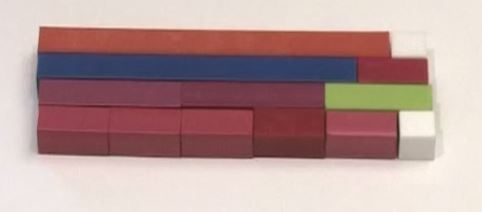
\includegraphics[width=0.75\textwidth]{rods.JPG}
  \centering
  \caption{A set of Cuisenaire\textsuperscript{\textregistered} Rods in use \cite{24Lesnom77:online}}
  \label{fig:rods}
\end{figure}

A set of rods consists of different-coloured cuboids, each colour of a different length, the smallest of which represents one unit. The rest of the rods are sized in multiples of this unit up to the longest rod, usually of size 10. Pupils are taught how different sized rods can be placed end-to-end in order to reach the target summation result, and are encouraged to find several alternate combinations of rods that add to the result, as demonstrated in Figure \ref{fig:rods}. This is a physical representation of number bonds, as the pupil can learn to associate a 7-rod (a rod of length 7) and a 3-rod forming a line of length 10 units with the mathematical concept that $7+3=10$. \\

The current disadvantage of the use of these rods is that in a class of dozens of students, it can be difficult for a teacher to monitor and track student progress. The teacher can survey the classroom, but is not capable of giving every student constant attention, so inevitably, poor progress sometimes goes unnoticed and students may fall behind without extra support. Additionally, students need to make a record of the work they have done, which can be difficult with the existing rods, as their use does not necessarily involve any written work.
\chapter{Project Specification}

Cuisenaire\textsuperscript{\textregistered} Rods \cite{TheCuise14:online} are an educational tool used in primary school mathematics classes to aid in the learning of, among other things, 'number bonds'. These are simple addition sums typically resulting in a round number like 10 or 20, such as $7+3=10$, which children learn as a foundation for more complex mathematical relationships. These are an important part of the Key Stage One (ages 5-7) curriculum in the UK, as recommended by the British Government \cite{Mathemat26:online}. 

\begin{figure}[h] 
  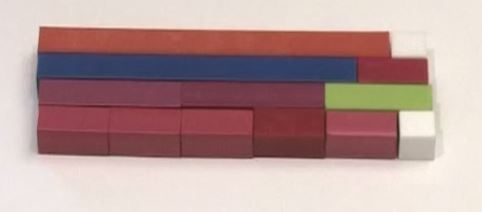
\includegraphics[width=0.75\textwidth]{rods.JPG}
  \centering
  \caption{A set of Cuisenaire\textsuperscript{\textregistered} Rods in use \cite{24Lesnom77:online}}
  \label{fig:rods}
\end{figure}

A set of rods consists of different-coloured cuboids, each of a different length, the smallest of which represents one unit. The rest of the rods are sized in multiples of this unit up to the longest rod, usually of size 10. Pupils are taught how different sized rods can be placed end-to-end in order to reach the target summation result, and are encouraged to find several alternate combinations of rods that add to the result, as demonstrated in Figure \ref{fig:rods}. This is a physical representation of number bonds, as the pupil can learn to associate a 7-rod (a rod of length 7) and a 3-rod forming a line of length 10 units with the mathematical concept that $7+3=10$. \\

The current disadvantage of the use of these rods is that in a class of dozens of students, it can be difficult for a teacher to monitor and track student progress. The teacher can survey the classroom, but is not capable of giving every student constant attention, so inevitably, poor progress sometimes goes unnoticed and students may fall behind without extra support. Additionally, students need to make a record of the work they have done, which can be difficult with the existing rods, as their use does not necessarily involve any written work. The aim of this project is to design and build a product that resolves this, by using a technologically-enhanced version of the rods which will allow the teacher to detect struggling pupils and provide assistance to them, as well as keeping an electronic record of all the students' sessions with the rods. They should do so by gathering data about the way the students are using the enhanced rods, such as time spent on an exercise, how many answers were found, and perhaps even more complex information like detecting patterns in which solutions were discovered. This data can be analysed to provide an overview of how the entire class is coping with the task.\\

The project is split into two halves: the software, including processing of data and user interfaces, is being completed by another student (Pierre Azalbert). The hardware, including the design and production of the rods, is the focus of this report.\\


Making the correct design choices will greatly affect the efficacy of the product. The final product will likely be used by publicly-funded schools, so costs should be kept low. The aim of the product is to make the teaching process easier for the teacher and to improve the learning experience for the pupils, so care should be taken to make the product as accessible as possible for both parties. This means keeping setup steps simple for teachers, and using human-computer interface (HCI) principles to ensure students find the product easy to use.


\chapter{Background}


\section{Cuisenaire\textsuperscript{\textregistered} Philosophy}
Background research began with discovering how Cuisenaire\textsuperscript{\textregistered} rods are used and why they are useful. John V. Trivett, in his article, \emph{The Cuisenaire Rods—Numbers in Colour}, from the Journal of the Association of Teachers of Mathematics \cite{johnv.trivett1962} talks about how abstracting the notation from the teaching of mathematics allows students to form conceptual instincts about ratios between values. He argues this is more valuable than committing equations and expressions to memory to be regurgitated during examinations. This idea is reinforced by Tony Wing in his article in the same journal, \emph{Working Towards Mental Arithmetic... And (Still) Counting}\cite{tonywing1996}, where he states that it is important for children to learn to play with the rods \say{before conventional number names and symbols are attached to them}.\\

This is something to keep in mind throughout the design process: we want to adhere to that principle of abstraction and not construct the rods in a way that would cause the children to treat them as numbers, for example, by having each rod's length written on it. \\

\section{Teacher Advice}

Further research was carried out by contacting primary school maths teachers who have made use of Cuisenaire\textsuperscript{\textregistered} rods, to ask them about the benefits of the rods and what could be improved. A criticism of the rods is that teachers need to record proof of students' work for administrative purposes, and the rods do not lend themselves to this very well because the children are required to draw diagrams of their solutions in workbooks, which takes considerable time from the exercise. This is a problem that our product will likely be able to solve, as an electronic system will be able to record every attempt a student makes at an answer, meaning that our records will be more detailed than what the children could draw themselves.\\

Another complaint was that, often, neither students nor teachers know how to properly make use of the rods when presented with them. This creates, for us, a task in human-computer interaction, as we will have to design a system that is intuitive to use with little mental effort required by the user. This includes being intuitive to set up (for teachers) and intuitive to operate (for children).\\

It was warned that students may not treat the product with care and so it should be able to withstand bending or general mistreatment at the hands of the children. This will inform our choice of material and construction method once we begin production. \\


\section{Similar Products}
Online searching yielded very few internet-enabled educational devices for the KS1 demographic, excluding educational applications for tablets and computers. This means that we will not be able to compare the hardware aspect of our product to existing designs, and will be setting precedents with some of our design choices. While this gives us the opportunity to explore and discover new methods of integrating technology into teaching, it does mean that the chance of our ideas being unsuccessful are increased, as we do not have a foundation of work to build upon. This effect can be mitigated via consultation of our contacts in schools and by working closely with our supervisor who can help guide our path.





%\chapter{Implementation Overview}
% Explain final product

\section{Rod}

\section{Board}

\section{Circuit}

\section{Power}

\section{Board to Hub Communication}

\section{Hub to Server Communication}
\chapter{Design Choices}
% Explain design decisions leading to final product


\section{Where should electronic complexity lie?}
\label{sec:complexity}

Some form of electronic device has to be used to identify the relative positions of the rods, in order to ascertain how the student has arranged them, but we have some choice in where this device exists. If we want to keep our product to be simply a set of rods, then the only place for the device is within the rods themselves. The rods would each need to be able to communicate with each other, to discern relative position, and also communicate with  a server for further processing.\\

Unfortunately, this solution brings several impracticalities. Firstly, the size of the rods has to be kept small, not only for storage purposes but also to allow the children to comfortably pick them up and work with them. We will try to keep our rods as close as possible to the original rods, which are about 1cm in diameter. This constrains the size of battery we could embed into them. They will have to be capable of transmitting and receiving wireless messages, and even perhaps perform some amount of processing, so their power consumption will be too high for a battery of that size. Charging the batteries would also be impracticable; consider a classroom of up to 30 students, each with a set of dozens of rods, and it becomes clear that the hassle of having to charge each device individually would outweigh any benefit of the product to a teacher.\\

Another issue concerns the identification of rods and their assignment to students: remember again that each student needs their own set of dozens of rods, and that any information these rods transmit will be attached to that child’s profile. The teacher would have to perform the frustrating and repetitive task of assigning each rod to a student, causing a considerable amount of inconvenience. Additionally, we must keep in mind that our target users are children, who may have the tendency to take rods from another student, misplace their own rods, or perhaps even throw rods around the classroom – all of these actions could cause sets of rods to be mixed together, leading to incorrect data being sent to the server, as progress from one student will be attached to the profile of another.\\

The last issue is economic: each of these rods will require several electronic components, including a processing unit and wireless transceivers, driving the cost of each unit up considerably. This is especially relevant as the smaller rods are easily lost in the classroom, so replacements would likely need to be purchased, increasing ongoing costs further.\\

An alternative solution to putting complexity in the rods is to design a playing board with which the rods can interact, and embed the majority of the electronics in that instead. The board would resemble a chess board, with grid squares guiding the placement of rods. The students arrange their rods on the board, which can identify the positions of the rods through some means, and communicate that data to the server. This alleviates all of the problems detailed above. The board is large and can house a larger battery than the rods, so there would be no power problem. There would only be one board per child so there are fewer devices to charge and much less work involved in assigning devices to children, also meaning that mixing of rods is not an issue, as it is the board which is unique to the child, not the rods. The cost to replace rods would be much lower as they would not contain as much electronics, and the overall cost would be lower as only the boards would require processing and communications equipment, as opposed to fitting one to every rod.\\ 

During an interview with a primary school teacher, we were informed that having a board may actually aid in the students’ learning, as having a grid could help them conceptualise how the rods fit together.\\

The choice was made to design a board with a 10x10 set of grid squares as this would allow rods to be placed in both the vertical and horizontal direction on the board, giving the product more flexibility. It was later decided that restricting use to only one direction would be more suitable, the reasons for which are explored further in Section \ref{sec:board}. This is why some of the design justifications may make reference to a 10x10 board.

\section{How should the board detect rod positions?}
\label{sec:detection}  


Having settled on the use of a board, the next design choice to be made is what technology it will make use of to detect where rods have been placed. The chosen method needs to have the following characteristics to be viable: it must be able to \textit{reliably} detect rods and their positions, as any errors may mislead and confuse the child, weakening the product’s effectiveness as an educational tool. It should keep \textit{cost} low, as there could be up to hundreds of these products in use at an institution, and since they will likely be using public funding they will be under budget constraints. It should keep \textit{power consumption} to a minimum to maximise the amount of use between charges. Lastly, it should remove as much \textit{complexity} from the rods as possible, for the reasons outlined in section \ref{sec:complexity}. \\

%%  Weight %%

\subsection{Weight}
\label{weight}

Rods could be given different weights, which are sensed by load sensors on the board. Each weight would be mapped to a different length of rod.\\

{
\setlength{\parindent}{0pt} % Remove paragraph indents within this block

\textbf{\textit{Reliability:}} It may be difficult to distinguish between the weight of a rod and the weight from the child touching the board, which could lead to false readings. However, under good conditions it should be possible to distinguish between rods well.\\

\textbf{\textit{Cost:}} The cost of the rods will likely be low, as they will just require weighting, however the board will require a load sensor in every grid square. The load sensor would need to be small enough to fit into a square around $2cm^2$ in area, and be sensitive enough to detect weighted rods light enough for a child to safely play with. A preliminary search revealed that components meeting those specifications would cost tens of pounds  \cite{ref:loadsensor}. Considering we are using a 10x10 board, purchasing 100 of these components would increase the cost to unacceptable levels.    \\

\textbf{\textit{Power Consumption:}} The datasheet of a suitable sensor \cite{MICROSWI18:online} states a typical voltage requirement of $10V$, and an input resistance of $5k\Omega$. Using $P=\frac{V^2}{R}$ we can determine a power usage of $0.02W$. 100 of these components would then draw 2W, which is relatively high, but could be acceptable depending on the battery used. \\

\textbf{\textit{Rod Complexity:}} The rods will not need any electronics, just some weighted material, so the complexity is quite low.\\
}

%%  Magnets %%

\subsection{Magnetic Fields}
\label{magnets}

Magnets of varying strength could be inserted into rods to be detected by Hall effect sensors in the board. Each strength would be mapped to a different length of rod. \\

{
\setlength{\parindent}{0pt} 

\textbf{\textit{Reliability:}} In terms of magnetic stability, a system using magnets could be quite reliable, as rare earth magnets can be used for several years without their strength diminishing \cite{Permanen88:online}. The limiting factor would be the operation range of the sensors, as too high a range would mean it could mistakenly detect a field from a neighbouring rod. The activation distance of a representative sensor was found to be up to 1-2cm \cite{47017pdf16:online}, which is slightly too high for our purposes. There is also the problem that since dipole magnetic fields follow the inverse-cube law \cite{Theinver11:online}, the strength of the field as detected by the sensor will increase as the magnetic rod approaches the sensor, so the sensor may mistake the rod for one of a weaker strength as it is being placed. \\

\textbf{\textit{Cost:}} A search for the least expensive sensor that meets the specifications most closely yielded a result \cite{A1318LUA39:online} which is priced at over £1 per unit, making it too expensive for our purposes, as 100 would be required for our 10x10 board. \\

\textbf{\textit{Power Consumption:}} The datasheet of a representative sensor \cite{47017pdf16:online} suggests a power usage of 0.04-0.24W per unit (4-24V $\cdot$ 10mA) and with 100 units, that would bring power usage to 4-24W, which is too high to maintain.   \\

\textbf{\textit{Rod Complexity:}} The rods would be kept quite simple, as they would just require a magnet inserted into them. However, it would be important for the strength of the rods to be precise to distinguish rods from each other.\\
}

%%  RFID %%

\subsection{RFID}
\label{rfid}

Passive RFID chips could be inserted into the rods, and RFID sensors into the board. Each RFID chip would contain identifying information about the rod it is in. When a rod is placed on the board, its RFID chip is powered and the data is read, and sent to the server. \\

{
\setlength{\parindent}{0pt} 

\textbf{\textit{Reliability:}} Our requirements are such that the range of detection of a rod should be very small, no more than a centimetre, as otherwise neighbouring grid squares could erroneously detect nearby rods and send false data to the server. A search for RFID products that operate in this range found no suitable results, which indicates RFID is not tailored to the precision detection needed for this project.\\

\textbf{\textit{Cost:}} An example of one of the shortest range components of the correct dimensions retails at between £5-14 per unit \cite{RITRPR9U23:online}; while this is much cheaper than the load sensor described above, it would still raise the price of the product to an unacceptable level given the quantity of boards/rods needed for a classroom.\\

\textbf{\textit{Power Consumption:}} Since the components in the rod are passive, they would draw a minimal amount of power, powered by the reader. A suitable reader \cite{AS3991BQ49:online} is listed to draw 0.558-1.705W. 100 of these would draw an unmanageable amount of power. \\

\textbf{\textit{Rod Complexity:}} Since this solution requires inserting electronics into the rods, the complexity is quite high. This increases the chance that something may fail and rods will need to be replaced. Another problem is that readings will be inaccurate until the fault is discovered, which may take some time. \\
}


%%  RGB %%

\subsection{RGB Light}
\label{rgb}

Each grid square of the board could contain an RGB LED and a photodiode; the LED would flash periodically and the photodiode would measure the frequency of the reflected light. Since each rod is of a distinctly different colour, each would produce a different reflected frequency.\\

{
\setlength{\parindent}{0pt} 

\textbf{\textit{Reliability:}} This method has the potential for very good reliability, as there are few enough different sizes of rod such that each can have a distinct colour, which reduces the possibility of a false reading. However, it is unclear how such a system might respond to a different object like a child's hand being placed on the board. \\

\textbf{\textit{Cost:}} The cost of the components for this design is quite high: 100 pairs of a suitable photodiode \cite{KPS5130P52:online} and LED \cite{L154A4SU86:online} would cost over £150.  \\

\textbf{\textit{Power Consumption:}} Taking the typical operating voltages of each colour of the RGB LED (1.95V. 3.3V and 3.3V for red, green and blue, respectively) at the typical current draw (20mA), constant powering of an LED would require $(1.95 + 3.3 + 3.3) \cdot 0.02 =$ 0.171W. Assuming a 25\% duty cycle, since the LEDs will be flashing, this is reduced to 0.04275W. 100 of these would then draw 4.275W, which is relatively high.\\

\textbf{\textit{Rod Complexity:}} This method requires adding nothing at all to the rods: since the solution works by sensing colour, the rods would be simply coloured as they are in the original set of rods.\\
}

%%  Resistors %%

\subsection{Shorting Resistor Chains}
\label{resistors}

Each row on the board could be linked to a long series chain of resistors of known values, and the rods themselves could contain a wire connecting two contacts, on either end of the rod. Each row would have its own chain, connected in parallel to the other chains, with a contact on each grid square connected to a node along the chain. When the rod is placed on the board, its contacts would connect to contacts on the board, shorting a number of resistors in the board relative to the rod's length. The change in voltage at the different nodes in the line could be used to detect if and where a rod is placed. Figure \ref{fig:unitrod} demonstrates more clearly how this could work.\\

{
\setlength{\parindent}{0pt} 

\textbf{\textit{Reliability:}} This solution will be very reliable as long as the contacts are designed in such a way that a child could not short resistors without a rod, which would produce a false reading. Another requirement is that the voltage level be high enough so that every node in the chain of resistors is sufficiently different and distinguishable.\\

\textbf{\textit{Cost:}} The only component required is resistors, which are orders of magnitude cheaper \cite{CFR25J1024:online} than the resources required for the alternative solutions.\\

\textbf{\textit{Power Consumption:}} The power consumption will be low: assuming the board will be controlled by a microcontroller with a 5V rail powering 10 parallel chains of resistors each totalling $2K\Omega$ (meaning the overall resistance is $200\Omega$), a $P=\frac{V^2}{R}$ calculation reveals a power usage of $0.125W$, which is quite acceptable.  \\

\textbf{\textit{Rod Complexity:}} The rods will be kept relatively simple, as they will just need a wire between the two contacts inside them, however the design of the contact could increase complexity.\\
}


Table \ref{tab:method_comparison} summarises each method's adherence to the specification with colour,  green representing a strong adherence, red representing a weak adherence, and yellow representing a moderate adherence. \\

\begin{table}[H]
\centering
\begin{tabular}{llllllllll}
                  & Weight                   && \multicolumn{1}{p{2cm}}{\centering Magnetic \\ Fields}         && RFID                     && RGB Light                && \multicolumn{1}{p{2cm}}{\centering Resistor \\ Chains}          \\
Reliability       & \cellcolor[HTML]{FFFE2F} && \cellcolor[HTML]{FD6864} && \cellcolor[HTML]{FD6864} && \cellcolor[HTML]{67FD9A} && \cellcolor[HTML]{67FD9A} \\
Cost              & \cellcolor[HTML]{FD6864} && \cellcolor[HTML]{FD6864} && \cellcolor[HTML]{FD6864} && \cellcolor[HTML]{FCFF2F} && \cellcolor[HTML]{67FD9A} \\
Power Consumption & \cellcolor[HTML]{FCFF2F} && \cellcolor[HTML]{FD6864} && \cellcolor[HTML]{FD6864} && \cellcolor[HTML]{FFFE2F} && \cellcolor[HTML]{67FD9A} \\
Rod Complexity    & \cellcolor[HTML]{67FD9A} && \cellcolor[HTML]{67FD9A} && \cellcolor[HTML]{FD6864} && \cellcolor[HTML]{67FD9A} && \cellcolor[HTML]{FCFF2F}
\end{tabular}
\caption{Method Comparison Summary}
\label{tab:method_comparison}
\end{table}


 
Considering the above comparison, the best solution is the resistor chains; it is comparatively inexpensive, uses comparatively low power, and does not rely on any complex technologies so has high reliability. The complexity of the rods is slightly increased due to the need for contacts, but faults with these should be more apparent than faults with electronics embedded in a rod, and in the event of a fault, replacement rods will not incur significant cost.\\



%%				%%
%%  Prototyping	%%
%%				%%

\section{Prototyping}

\subsection{Controller}
To control the reading of data from the resistor chains, it was decided to make use of an Arduino microcontroller board \cite{ArduinoH73:online}. This was mainly because of its ease of use, and active community of users who can provide support during the prototyping process. The Arduino board provides an interface to external hardware via GPIO (General Purpose Input/Output) pins that can be used to read the voltages along the chain of resistors, and has a 5V source that can be used to power the prototype. 

\subsection{Determining Rod Placement}
\label{sec:voltages}
Prototyping began with the construction of two parallel simple resistor chains \ignore{(shown in Figure \ref{fig:simple_resistor})} to learn to use the Arduino and to get some intuition on how rod placement could be ascertained from the measured voltages. 

\ignore{
\begin{figure}[H]
	\begin{center}
	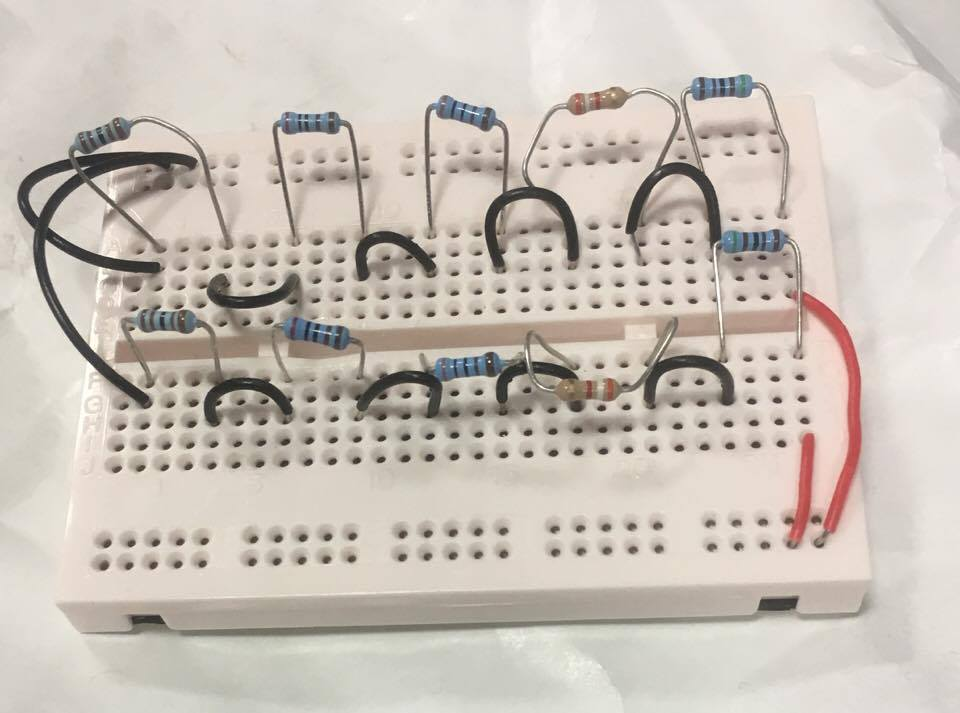
\includegraphics[width=0.75\textwidth]{simple_resistor_chain.jpg}\\
  	\caption{Parallel Resistor Chains}
    \label{fig:simple_resistor}
    \end{center}
\end{figure}
}

This first attempt incorporated the use of differing resistors down the chain, as in Figure \ref{fig:5r} (although it was later realised that using equal resistors would be better suited as they would give uniform increments of voltage at each node along the chain). A wire was used to connect two of the labelled nodes A-E to represent the functionality of the rod shorting resistors. Voltage was measured at two points along the chain to see if each different position of the rod along a chain could produce a unique pair of voltages that could be used to identify that position.  \\



\begin{figure}[H]
	\begin{center}
	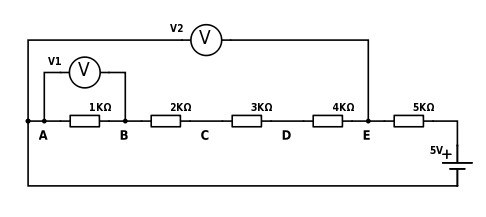
\includegraphics[width=0.8\textwidth]{5r.png}\\ 
  	\caption{Simple prototype with labelled nodes}
    \label{fig:5r}
    \end{center}
\end{figure}



\begin{table}[H]
\centering
\begin{tabular}{c|ccccc}
\cline{2-6}
                                 & \multicolumn{1}{c|}{\textbf{A}}                 & \multicolumn{1}{c|}{\textbf{B}}                 & \multicolumn{1}{c|}{\textbf{C}}                 & \multicolumn{1}{c|}{\textbf{D}}                 & \multicolumn{1}{c|}{\textbf{E}}                 \\ \hline
\multicolumn{1}{|c|}{\textbf{A}} & \multicolumn{1}{c|}{\cellcolor[HTML]{C0C0C0}}   & \multicolumn{1}{c|}{0, 3.18}                    & \multicolumn{1}{c|}{0, 2.88}                    & \multicolumn{1}{c|}{0, 2.17}                    & \multicolumn{1}{c|}{0, 0}                       \\ \cline{1-1} \cline{3-6} 
\multicolumn{1}{|c|}{\textbf{B}} & \cellcolor[HTML]{C0C0C0}                        & \multicolumn{1}{c|}{\cellcolor[HTML]{C0C0C0}}   & \multicolumn{1}{c|}{0.41, 3.05}                 & \multicolumn{1}{c|}{0.53, 2.47}                 & \multicolumn{1}{c|}{0.87, 0.87}                 \\ \cline{1-1} \cline{4-6} 
\multicolumn{1}{|c|}{\textbf{C}} & \cellcolor[HTML]{C0C0C0}                        & \cellcolor[HTML]{C0C0C0}                        & \multicolumn{1}{c|}{\cellcolor[HTML]{C0C0C0}}   & \multicolumn{1}{c|}{0.44, 2.89}                 & \multicolumn{1}{c|}{0.66, 1.89}                 \\ \cline{1-1} \cline{5-6} 
\multicolumn{1}{|c|}{\textbf{D}} & \cellcolor[HTML]{C0C0C0}                        & \cellcolor[HTML]{C0C0C0}                        & \cellcolor[HTML]{C0C0C0}                        & \multicolumn{1}{c|}{\cellcolor[HTML]{C0C0C0}}   & \multicolumn{1}{c|}{0.48, 2.73}                 \\ \cline{1-1} \cline{6-6} 
\multicolumn{1}{|c|}{\textbf{E}} & \cellcolor[HTML]{C0C0C0}{\color[HTML]{333333} } & \cellcolor[HTML]{C0C0C0}{\color[HTML]{333333} } & \cellcolor[HTML]{C0C0C0}{\color[HTML]{333333} } & \cellcolor[HTML]{C0C0C0}{\color[HTML]{333333} } & \cellcolor[HTML]{C0C0C0}{\color[HTML]{333333} } \\ \cline{1-1}
\end{tabular}
\caption{Voltages (V1, V2) when two nodes are connected by a wire}
\label{tab:5r_voltages}
\end{table}

The values in Table \ref{tab:5r_voltages} show the voltages at V1 and V2 when each pair of nodes is connected. It is apparent that every combination of connected nodes does produce a unique pair of voltages, which proves that it is possible, in principle, to identify rods based on the voltages of the nodes. This experiment was a proof-of-concept, as it only used 5 resistors, but the real prototype needs at least 10 resistors to detect rods of up to size 10.\\

\subsection{The Problem with the Unit Rod}

At the end of Section \ref{sec:voltages} it was proposed that at least 10 resistors would be needed per chain to detect rods of up to size 10; while this is true, it overlooks the necessity to detect unit rods, of size 1. The assumption is that each node in the resistor chain is connected to a grid square on the board, and that rods connected to two nodes along a chain can short the resistors between those two nodes when connected to the board. However, a unit rod spans only one grid square, meaning that it is only connected to one node, and so cannot short any resistors. Figure \ref{fig:unitrod} demonstrates why this is the case. Note that the representations of the wires connecting the rods and the resistor chain are symbolic and do not represent what the actual connections would look like. \\

\begin{figure}[H]
	\begin{center}
	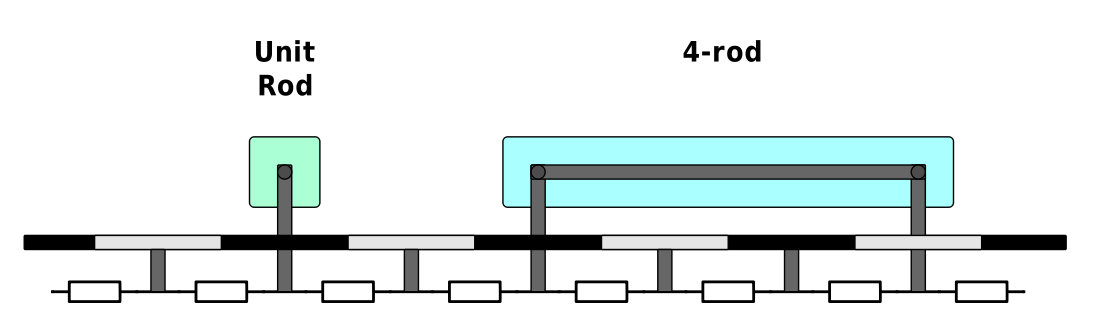
\includegraphics[width=0.8\textwidth]{unitrod.png}\\ 
  	\caption{Cross-sectional view of board}
    \label{fig:unitrod}
    \end{center}
\end{figure}

The chosen solution to this problem was add a double connector to the unit rod, so that it can connect to two nodes and short a resistor. This means that twice as many resistors are required along a chain, but allows us to detect unit rods without affecting the detection of the other sizes. Figure \ref{fig:doubleunitrod} demonstrates how doubling the number of resistors achieves this.\\

\begin{figure}[H]
	\begin{center}
	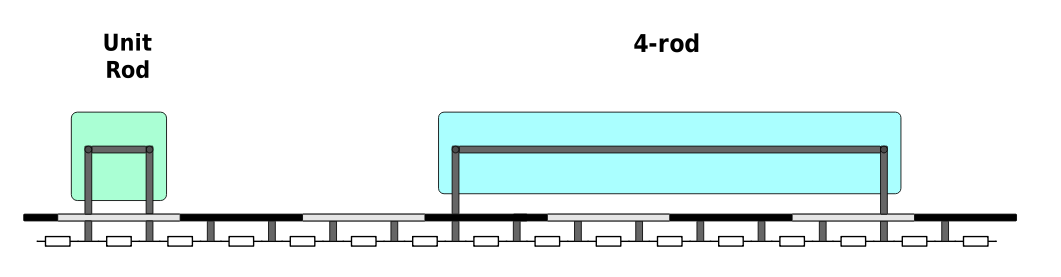
\includegraphics[width=\textwidth]{doubleunitrod.png}\\ 
  	\caption{Cross-sectional view of board with double resistor chain length}
    \label{fig:doubleunitrod}
    \end{center}
\end{figure}

%Two-value measurement table\\ 
%Why it wasnt suitable, needed to measure every node instead

\subsection{Practicalities in Data Measurement}

\par Taking only two voltage measurements worked well in the proof-of-concept from Section \ref{sec:voltages}, but when the same method was applied to a resistor chain of size 20, the voltage values measured were much less distinguishable from each other. This is because when the number of resistors is increased, the voltage across each is smaller, so shorting one makes less of a difference to the measured voltage, and thus a distinction between states is less easily made. \\

The solution to this was to measure the voltage at every node in the chain, and make use of the increased information to make a more accurate inference of the positions of rods. With so many nodes being measured, it would not be possible to connect each directly to the Arduino's limited GPIO pins. Instead, multiplexers are used to direct all measurements to a single pin. The CD4051BE 8:1 multiplexer \cite{CD4051BE27:online} was chosen instead of available 16:1 multiplexers, because although more 8:1 units would be required than 16:1 units to meet our needs, its relatively low price meant it was still the more economic choice. The method for mapping the measured voltage values to rod placements is detailed in Section \ref{sec:rods}. \\

Having decided on the detection method, the project can now be separated into six components which comprise the final product. These include the construction of the board and rods themselves, the circuitry used inside the board, the software that controls the processing of the data gathered by the circuit, the method used to power the circuitry, and the process of communicating the information from the board to the server for further processing. The design choices that play a part in each of these components are justified below, as well as explored paths that turned out to be unsuccessful.\\ 


%		%
%  Rods %
% 		%


\section{Rods}
\label{sec:rods}
To recap the specifications for the rods, they should be similar in size and shape to the original rods (1cm\textsuperscript{2} cross-sectional area cuboid), and be durable enough to withstand any mistreatment by the children. They also need to have some contacts that can interface with the board, and act as a short circuit when connected. 


\subsection{Construction Method}
\label{sec:Construction_Method}
The choice of construction method was based upon the precision and durability the method could offer. Precision is needed to create uniformly-positioned spaces for contacts, so that the rods line up with the grid squares on the board, and high durability is needed for the product to stay intact even after heavy use by children. \\

Advice from Imperial College Robotics Society (ICRS) and the Imperial College Advanced Hackspace (ICAH) led to deciding between using either 3D printing, or laser cutting. 3D printing is a manufacturing process that resembles conventional paper printers, but instead of applying ink to a page, a 3D printer extrudes material  (usually some form of plastic) through a nozzle on to a surface, repeatedly applying more extruded material atop previous layers to  form a physical object. Laser cutting, conversely, involves cutting a design into a sheet of material, by directing a high-powered laser to melt or burn the edges of the design. \\

The choice was made to use 3D printing, as it allows for more complex features that would likely be necessary for incorporating the electrical contacts in the design. For example, a laser cutter is not able to make cuts of varying depth in the material, so any recesses in the design would require cutting several layers of the design separately, then gluing them together. Using a 3D printer removes the need for this excessive labour. \\

After having chosen 3D printing as the construction process, the next decision was to choose the material that would be used. It was advised that the two most commonly-used materials are PLA (Polylactic Acid) and ABS (Acrylonitrile Butadiene Styrene), and that it would be best to select one of these, since colleagues in ICAH/ICRS have most experience with these, which would make it easier to get assistance in the event that problems arise. It was also noted that PLA is more brittle than ABS, and is more prone to snapping when bent, but other than that, there is no major differences that should cause concern for the purpose of this project. This information is corroborated by other sources found online \cite{PLAvsABS47:online}\cite{TheDiffe59:online}, so it was decided that ABS would be the material of choice. \\



\subsection{Conductive Material}
\label{sec:conductivematerial}
To provide a short circuit, the rods require some conductive material to be embedded inside, connecting the two contacts. The resistance of this material should be as low as possible in order to provide a short circuit.

\subsubsection{Conductive 3D Printing Filament}
The first idea was to take advantage of the fact that a 3D printer was being used to produce the rods, and insert a conductive material as part of that process. A company named Proto-Pasta produces a conductive filament \cite{Composit79:online} which seemed an appropriate tool to use. A model of the rod with a conductive centre can be seen in Figure \ref{fig:tenrodrender}. The rod was designed to have a non-conductive outer layer (shown in red) with the only exposed conductive material (black) being the locations where the contacts would be installed. This design was chosen over a rod made from purely conductive material to ensure that the nodes corresponding to the length of the rod were the first and only nodes to be connected, as opposed to connecting every node in-between as the rod is placed, since there is a chance that an in-between node would be registered as connected before the end nodes, which could produce erroneous data. Note also that there is space for a contact on four faces, to avoid the need for the child to find the right orientation before placing a rod.

\begin{figure}[H]
	\begin{center}
	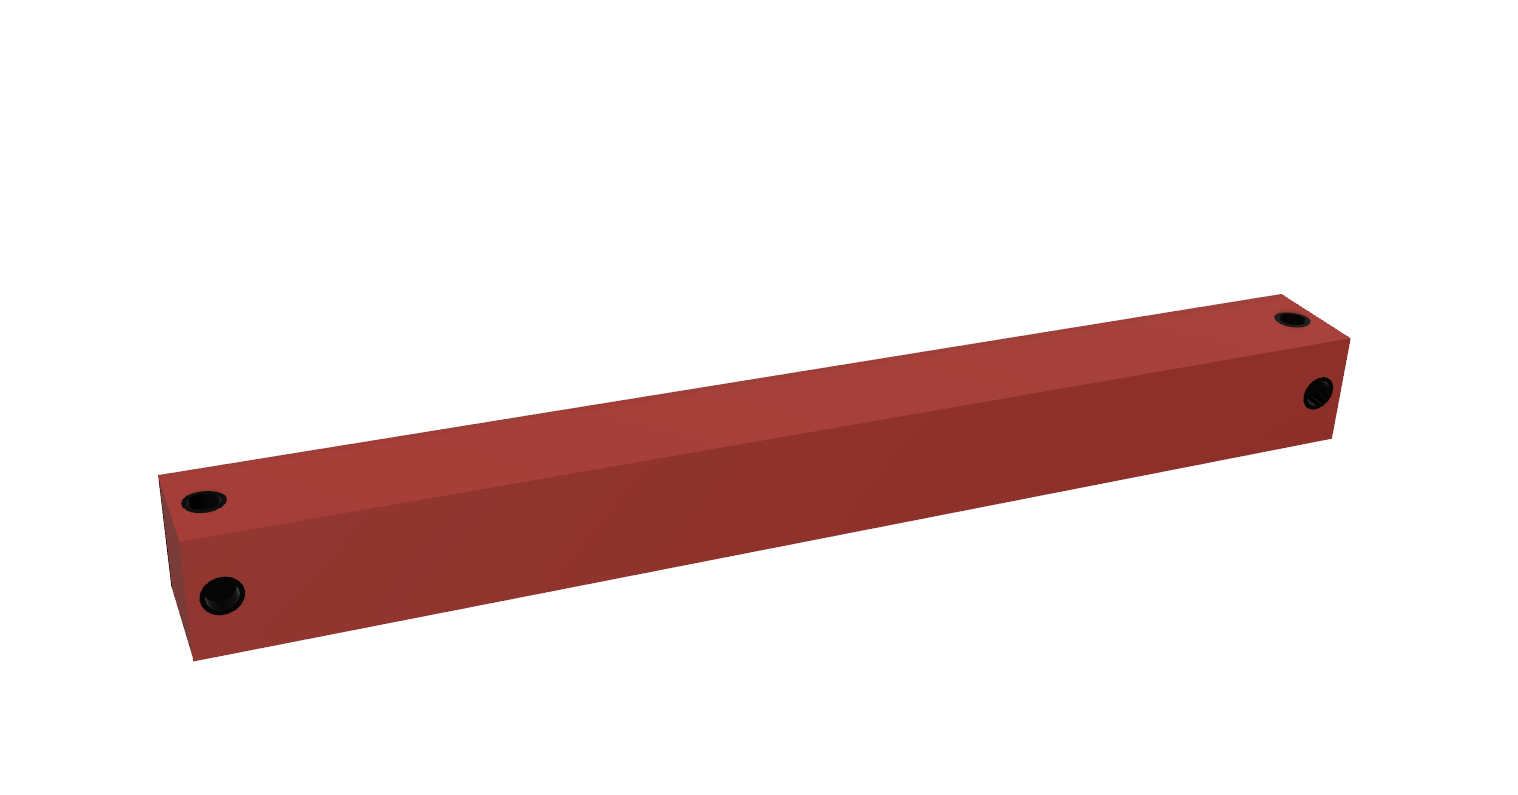
\includegraphics[width=\textwidth]{tenrod_render.png}\\ 
  	\caption{Model of 10-rod with made with conductive filament}
    \label{fig:tenrodrender}
    \end{center}
\end{figure}


Working with the material was difficult, as the filament was rather brittle and had a tendency to snap, causing complications in the printing process. Despite this, the method had promise, until the first prototype rods were printed and their resistance was measured. Two rods were printed, one unit rod and a 10-rod, with resistances of around $100\Omega$ and $1K\Omega$, respectively. Remember that the rods have to act as a short for the chain of resistors in the board, and so the resistance of the rod should be much lower than that of the chain. This means the chain resistors would need to be in the megaohm range for the circuit to function properly. 

While this is theoretically feasible, it became apparent that with such a high resistance, the current running through the chain would drop too low for the multiplexers to be able to take a voltage reading. Therefore, the conductive filament was no longer a viable option.


%Why cant use it
\subsubsection{Embedded Wire}
The slightly less elegant, but more suitable method of manually embedding a wire inside the rod was what was finally chosen. While this requires more manual work, it was necessary to have as low a resistance as possible in order to allow the circuit to  function. 

\begin{figure}[H]
  \begin{subfigure}{.5\linewidth}
    \centering
    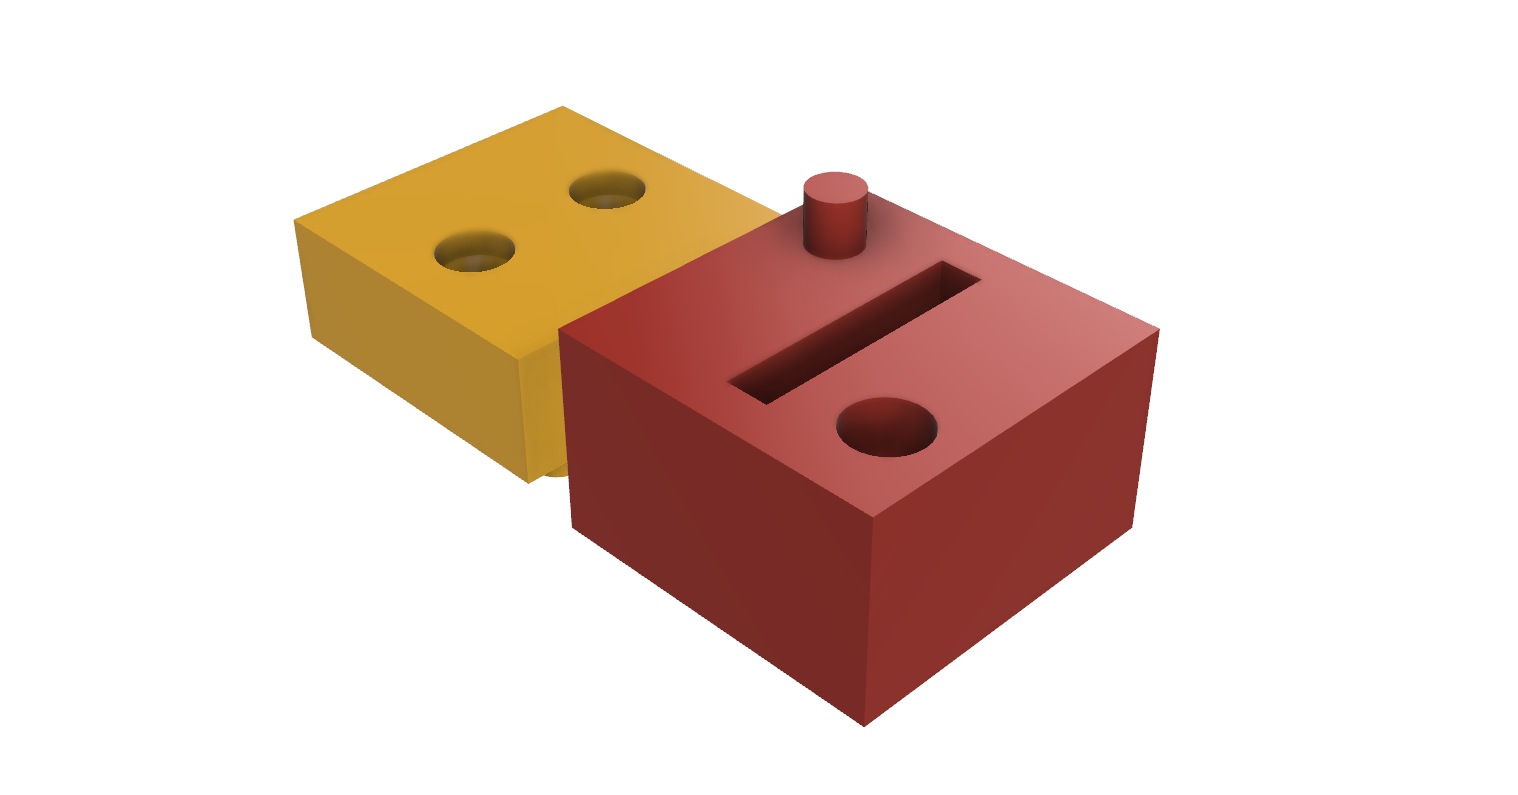
\includegraphics[width=\textwidth]{splitrod_viewhome}
    \caption{}
    \label{fig:splitrod_viewhome}
  \end{subfigure}%
  \begin{subfigure}{.5\linewidth}
    \centering
    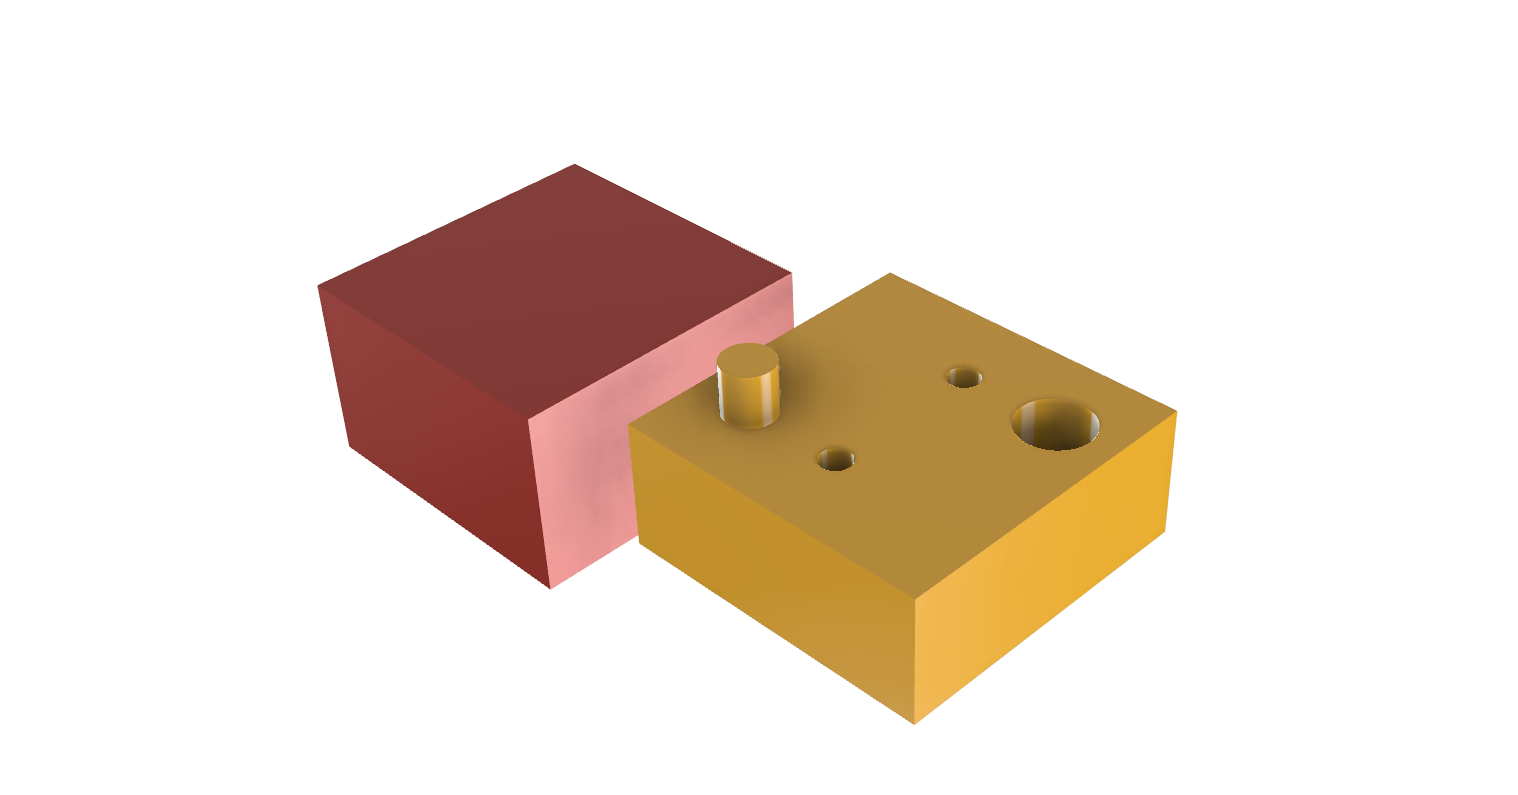
\includegraphics[width=\textwidth]{splitrod_viewbottomhome}
    \caption{}
    \label{fig:splitrod_viewbottomhome}
  \end{subfigure}\\[1ex]
  \begin{subfigure}{\linewidth}
    \centering
    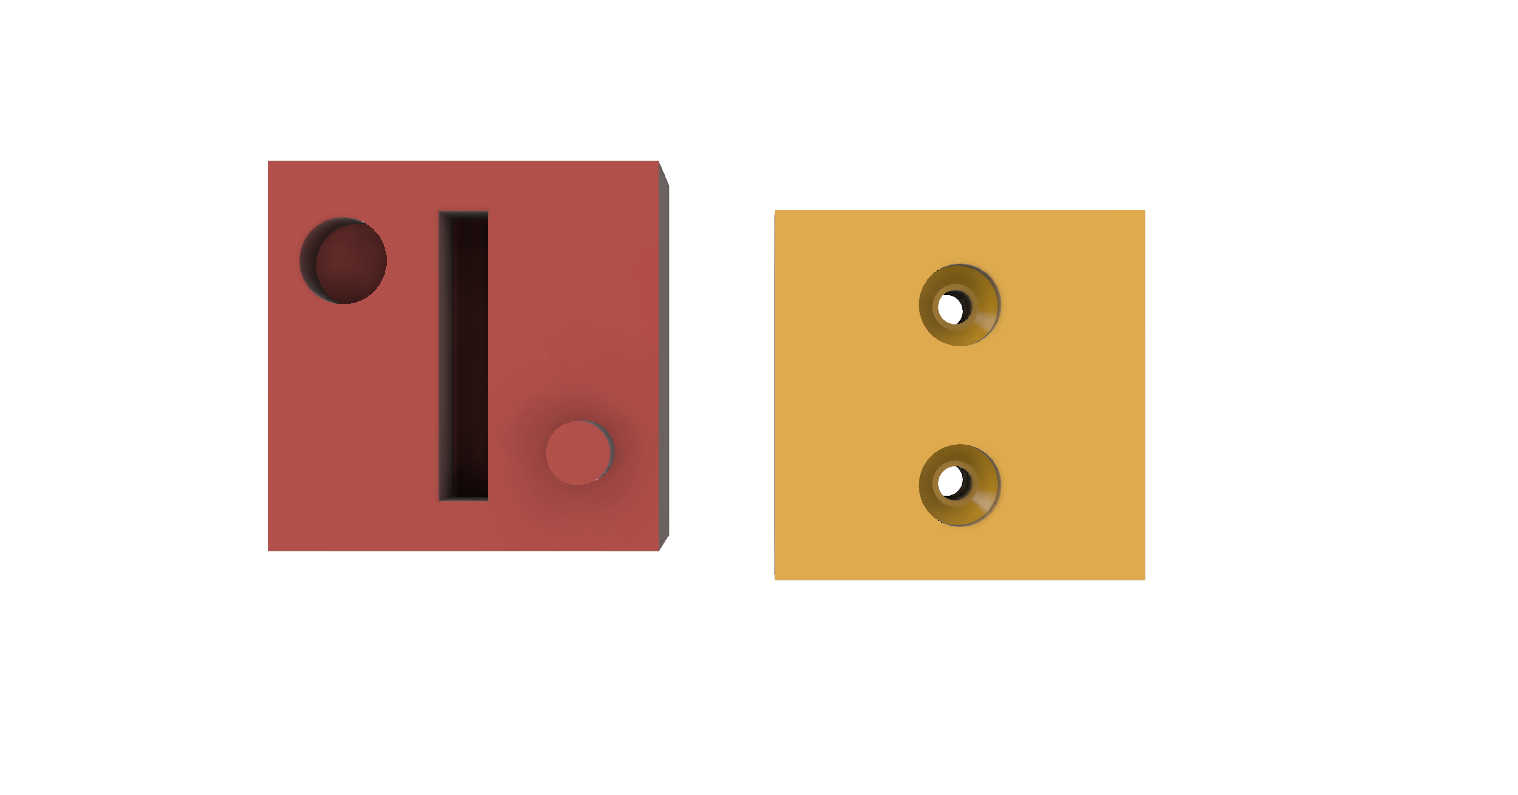
\includegraphics[width=0.5\textwidth]{splitrod_viewtop}
    \caption{}
    \label{fig:splitrod_viewtop}
  \end{subfigure}
  \caption{Rod parts viewed from different angles}
  \label{fig:splitrod}
\end{figure}


To embed the wire into the rod, construction was split into two parts, which can be slotted together after the wire is inserted. Figure \ref{fig:splitrod} shows the top (red) and bottom (yellow) pieces from different angles. The rectangular hole in the red part seen in Figures \ref{fig:splitrod_viewhome} and \ref{fig:splitrod_viewtop} is a space for the body of the wire to sit, and the two small holes in the yellow part seen in Figure \ref{fig:splitrod_viewbottomhome} are where the ends of the wires would be inserted in order to connect to the contacts. The two abscesses in the yellow part seen in Figures \ref{fig:splitrod_viewhome} and \ref{fig:splitrod_viewtop} are where the outward-facing magnetic contacts would be inserted. The cylindrical protrusion/hole seen at opposite corners of either piece are used to slot into one another, to encase the wire once it has been embedded. The hole was made slightly larger than the protrusion to leave some room for glue. \\


The disadvantage of using this method is that it makes it impractical to provide a contact on four faces of the rod, as was possible when using conductive filament. While unfortunate, this should not impact the usability of the product to a great degree, as the children should be able to recognise that the contacts on the rod should align with the contacts on the board. Hopefully, this visual cue will mitigate the problem.


\subsection{Electrical Contact}
\label{sec:electrical_contact}
One of the most difficult aspects of the project, from the perspective of manufacturing, was designing a way to attach electrical contacts on to the board and rod. The first step was to decide on the nature of the contacts, pertaining to size, shape, and contact mechanism. \\

The product should assist the child in aligning the rods to the grid squares on the board, to save the children from requiring the extra dexterity to do so themselves. Therefore, having contacts with come sort of locking mechanism would be preferable. However, it would not be beneficial to make the locking process too cumbersome or difficult to unlock, for example, with some form of clasp, since this could hinder the child's ability to easily add or remove rods as they experiment with different solutions. Using magnetic contacts on both the rod and board seemed like a good compromise, being able to guide the child's placement of the rod using the pull of the magnets, without requiring much force to remove the rod from the board. As long as the magnets are covered in metal, then they would be able to be connected to each other inside the rod, and connect to the contacts on the board to create a short. \\

Since the dimensions of the rods and grid squares are quite small, the magnetic contacts need to be small enough to fit on them. The chosen magnets \cite{MagnetEx80:online} were discs with a 2mm diameter and 1mm height, allowing two of them to comfortably fit onto a grid square or a unit cube face, which are the smallest areas of our product that require the two magnetic contacts. A concern may be that there is a choking hazard with such small parts on the product, but regulations as listed by the government Department for Business, Energy and Industrial Strategy \cite{Products54:online} note small parts to be of concern for ``toys intended for children under 36 months", and since the product is intended for children in Key Stage 1, who are typically aged 5-7 years old, we can be confident the small parts will not be an issue. \\

The next step was to consider how the magnets would be attached to the rod and board. The method used to achieve this is dependent on the conductive material used, so referring back to Section \ref{sec:conductivematerial} may assist the reader in better understanding these explanations. The main challenge was to attach the magnets to the conductive material inside the rod or board without the use of a soldering iron, because the extreme heat of the iron surpasses the magnets' curie point -- the temperature at which permanent magnetisation is lost. \todo[inline]{source} 

The first action taken was to research how existing products handled the same problem. One such existing products is Cubelets, manufactured by Moss Robotics -- these are modular blocks fitted with different sensors and actuators that can be combined to form electronic circuits. The blocks connect via magnetic contacts (shown in Figure \ref{fig:cubelets}), similar to how our rods and board would ideally connect. However, information on the methodology used to design these contacts was not publicly available, the conclusion being that some proprietary method is used. 

\begin{figure}[H]
	\begin{center}
	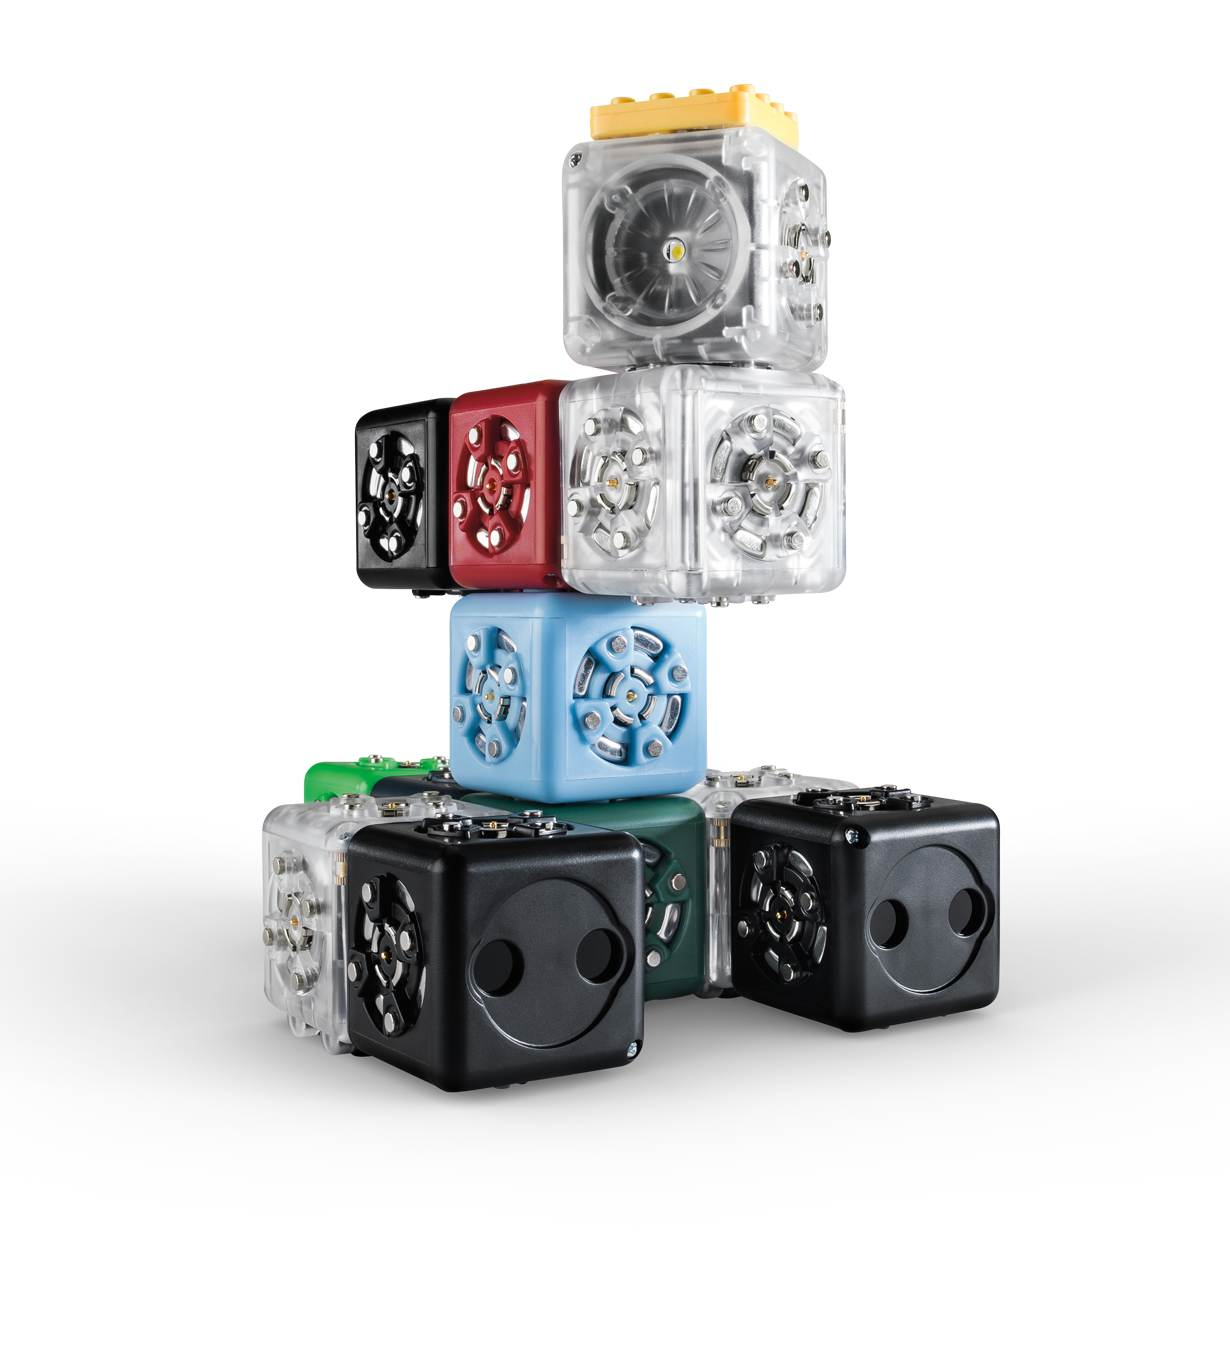
\includegraphics[width=0.5\textwidth]{cubelets.jpg}\\ 
  	\caption{Cubelets by Moss Robotics \cite{Cubelets52:online}}
    \label{fig:cubelets}
    \end{center}
\end{figure}

\subsubsection{Silver Paint as an Adhesive}

When the conductive material to be used was conductive 3D printing filament, the plan was to create an exposed area of the conductive material on the rod to which the magnet could be affixed, just as the black material is exposed in Figure \ref{fig:tenrodrender}. The adhesive used needed to be something which could, itself, conduct electricity, or else the magnet would be insulated from the conductive material. Seeking advice from colleagues led to the discovery of conductive adhesive \cite{ERSCP03B89:online}, a paint containing a high silver content that allows the flow of electricity. This paint could be used to coat the exposed area of the rod, to which the magnet would be attached. While the paint was certainly highly conductive, its success as an adhesive was limited; the paint itself easily adhered to surfaces, but this adhesion was not strong enough to keep the magnetic contact in place. \\

\subsubsection{Conductive Epoxy}

As detailed in Section \ref{sec:conductivematerial}, the use of conductive 3D printing filament was abandoned, and was replaced by a wire passing through the centre of the rod. The challenge was, now, to find a way to connect a wire to the magnet without the use of a soldering iron. Having seen the potential of the conductive silver paint, a similar product was experimented with: conductive epoxy. In general, epoxies are used to create strong adhesive bonds between materials, and often come in a liquid form that can be poured into cavities to mould around objects, to more effectively keep them in place. A conductive epoxy would, in theory, give the same conductive properties as the silver paint, but give much better adhesion, improving upon that drawback of the paint. 

The planned procedure was to put the wire and magnetic contact in place, in the rod, as the cross-section in Figure \ref{fig:rod_cross_section_nofill} and flood the cavity in the rod with the epoxy to connect the two. The wire would be fed through from the inside of the rod, through the holes in the yellow segment of Figure \ref{fig:splitrod_viewbottomhome}, and the magnets would fit in the recesses on the other side of the yellow segment, shown in Figure \ref{fig:splitrod_viewtop}. However, upon experimentation with the epoxy, it was found to be viscous and difficult to guide into the cavity correctly, much unlike the majority of regular epoxies. This difficulty was further exacerbated by the very small space the epoxy needed to fill, much of which was already occupied by the wires. This method may well have worked better for a larger cavity, but the available space is restricted by the size of the rod. Access to more precise tools may also have produced more successful results, as part of the difficulty arose from trying to hold all the small pieces in place while applying the epoxy. 

\begin{figure}[H]
	\begin{center}
	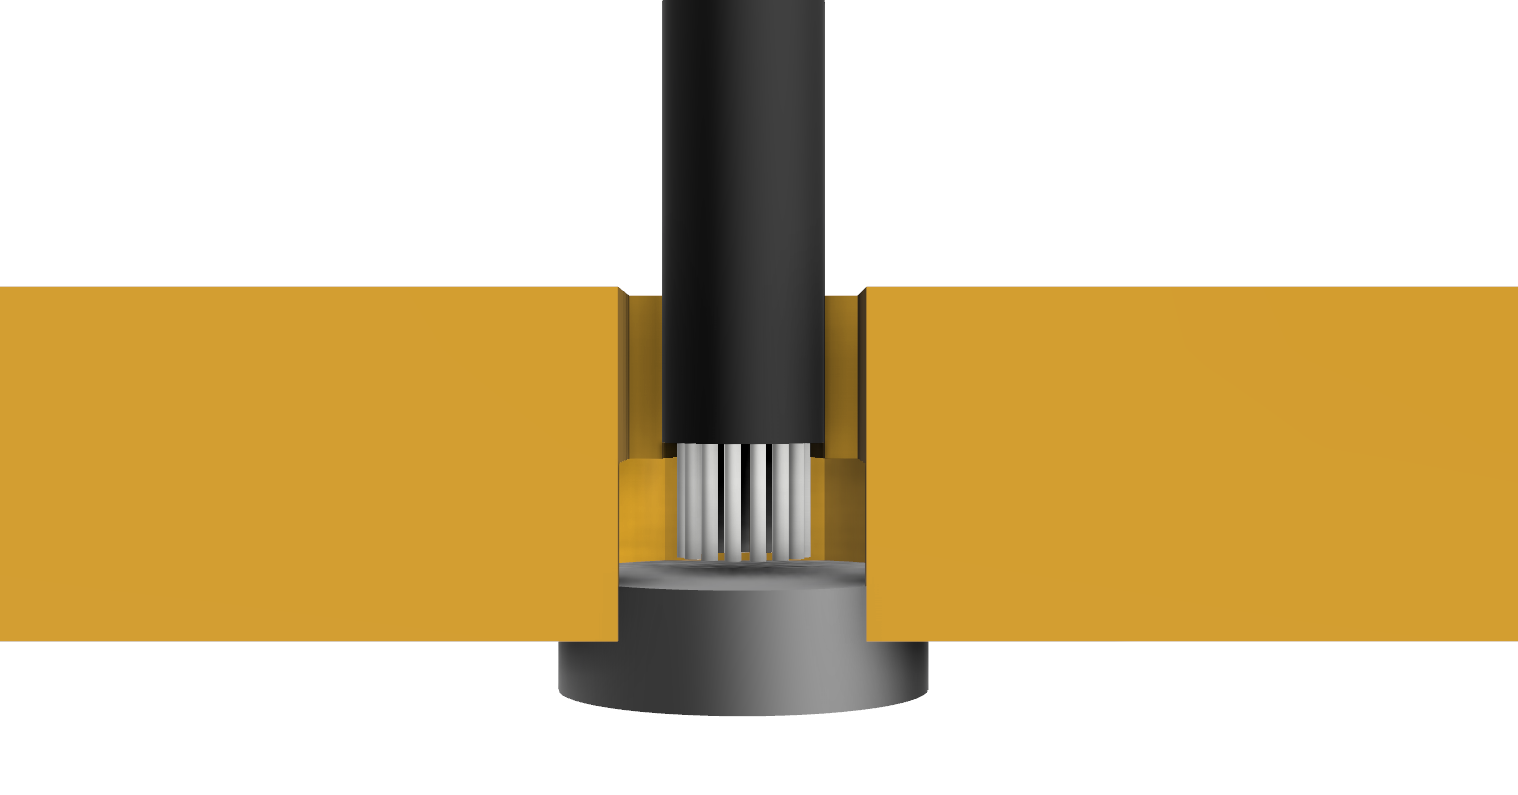
\includegraphics[width=0.6\textwidth]{rod_cross_section_nofill.png}\\ 
  	\caption{Cross-section of component showing magnet and wire in place in cavity}
    \label{fig:rod_cross_section_nofill}
    \end{center}
\end{figure}


It should be noted that concern about the possible dangers of using silver-based chemicals on is unnecessary, as although the epoxy materials are hazardous pre-application, the datasheet assures that ``The cured epoxy resin presents no known hazard".

\subsubsection{Silver Paint as a Cavity Filler}

As was discovered, the silver paint conducted well but did not have the adhesive strength to hold together the components. Additionally, the conductive epoxy had the strength to hold the components, but was too viscous to flood the cavity. So, an alternative solution was attempted: use the silver paint to fill the cavity, as it flows freely, and use a non-conductive glue to hold the components together, being careful not to insulate the contact from the wire with the glue. Figure \ref{fig:rod_cross_section_filled} demonstrates how this would be achieved. 
	
\begin{figure}[H]
	\begin{center}
	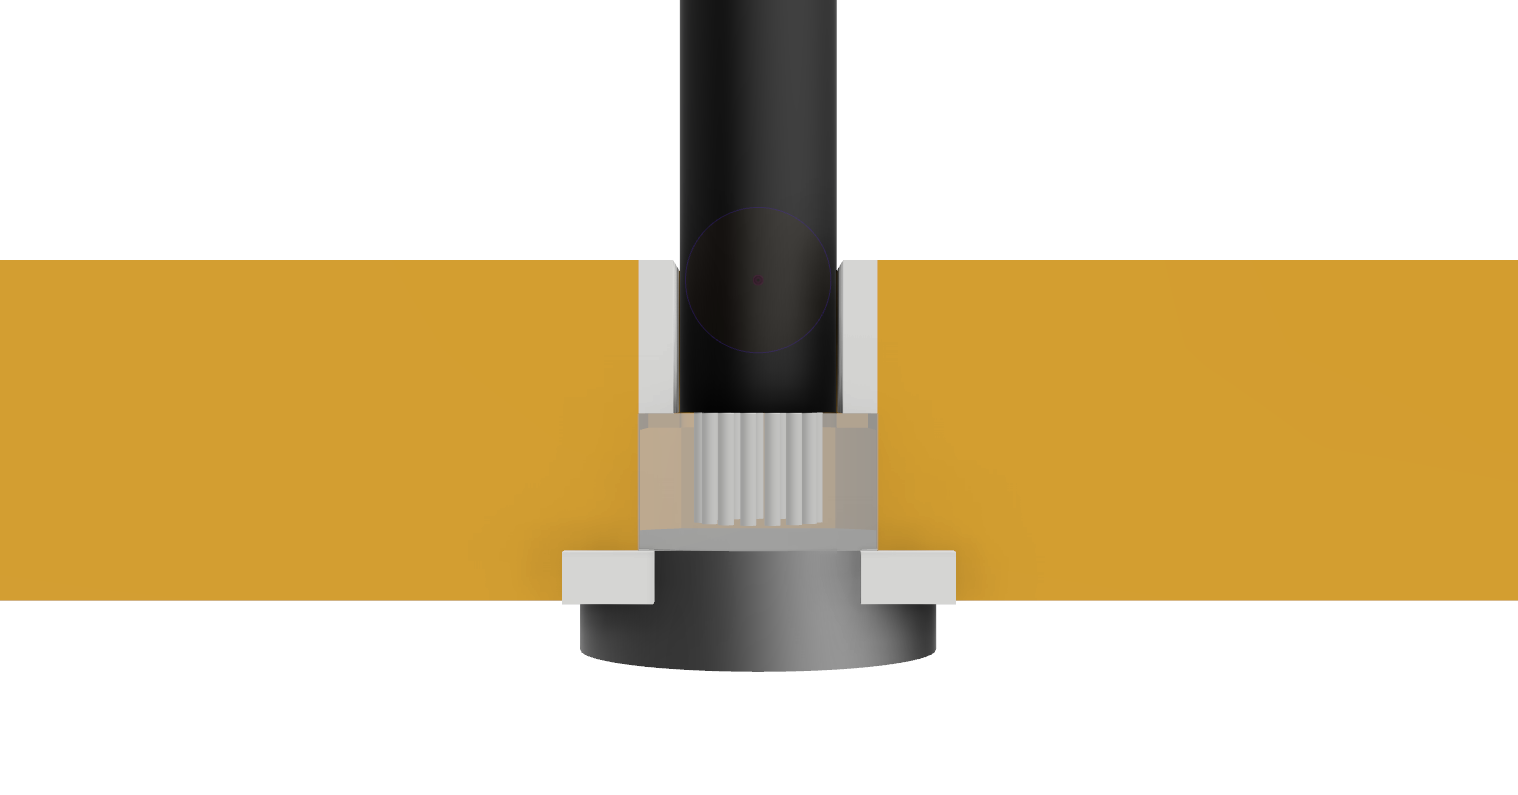
\includegraphics[width=0.6\textwidth]{rod_cross_section_filled.png}\\ 
  	\caption{Cross-section of cavity filled with silver paint (translucent grey) with glue (white) holding magnet and wire in place}
    \label{fig:rod_cross_section_filled}
    \end{center}
\end{figure}

While this method held promise, it was ultimated unsuccessful, again due to the level of precision required to apply glue to the small areas and hold the material in place. This could definitely be viable in circumstances where the appropriate equipment is available, but it was not practical in the university laboratory. 

\subsubsection{Header Pins}
\label{sec:header_pins}
After having failed multiple attempts to reliably create a bond between the wire and magnets, a less elegant but functional method was used, in the interest of keeping to deadlines. This method involves replacing the magnetic contacts on the board with female header pins, and inserting into the rods a row of male header pins, whose ends have been connected with a soldered wire. Figure \ref{fig:header_rod} shows the recess in the rod that has been left for the header pins. Then, the male pins can be inserted into the slots on the board in order to sort that row of resistors. While it is not what would ideally be in the final product, this solution was necessary in order to produce a proof-of-concept prototype for demonstration purposes.

\begin{figure}[H]
	\begin{center}
	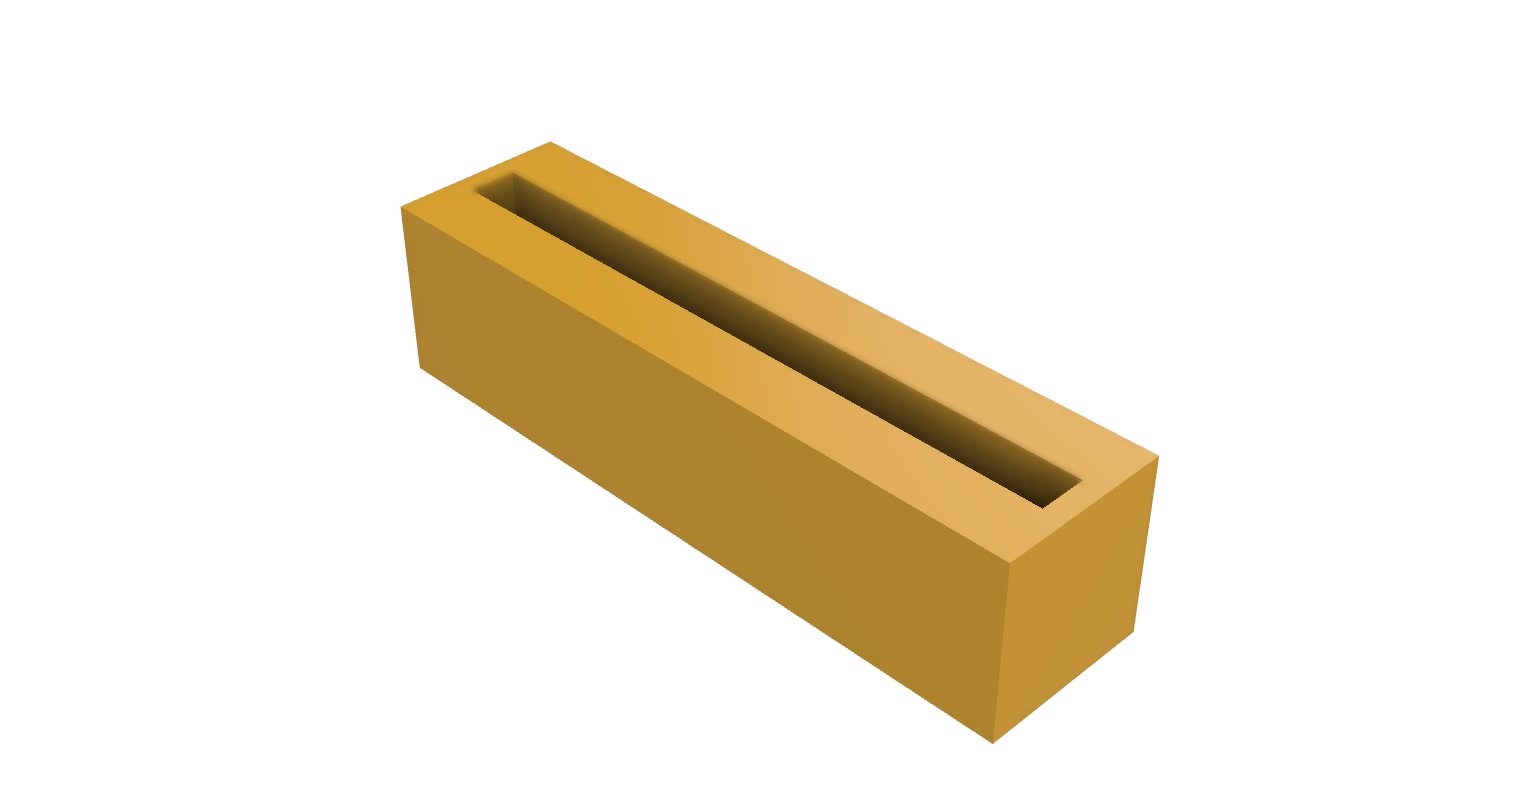
\includegraphics[width=0.8\textwidth]{header_rod.png}\\ 
  	\caption{Rod with space for header pins}
    \label{fig:header_rod}
    \end{center}
\end{figure}

\subsubsection{Alternative Ideas}
Due to time constraints, some potentially viable ideas were not explored. One such method was to solder the wire to a conductive metal foil, such as copper, then wrap the magnet in the foil before affixing it to the rod. The foil would not block the magnetic field, and would also allow an electrical connection to the wire without having to tamper with the magnet. However, there may have been problems with durability, as the foil could wear away with extended use, drastically shortening the life of the product. 

Another possible route would be to sandwich the end of the wire between two magnets, place the sandwich in a mould, and fill the mould with epoxy or hot glue, keeping one of the magnets exposed. This would form a secure contact between the wire and magnets, but would bring with it the expense of requiring double the magnets, and the added time and effort needed to create many moulds. It could also be subject to the same disadvantages seen earlier, pertaining to difficulties working with small components.


    
%			%
%   Board 	%
% 			%
    
\section{Board}
\label{sec:board}

The board needs to not only provide the functionality of a site for rods to be placed, but should also give visual cues to its users to help them understand how to properly make use of the product. Sections \ref{sec:Construction_Method}, and \ref{sec:electrical_contact} explain the design choices made with respect to construction of rods, and electrical contacts used, but the decisions made apply equally to the board. Section \ref{sec:header_pins} explained why the design of the board had to be changed to use header pins as opposed to magnetic contacts, but the sections below still outline the design process up to the time when that decision was made. 



\subsection{Grid Squares and Lane Markings}

As mentioned at the end of Section \ref{sec:complexity}, the choice was originally made to give the board a 10x10 grid for the children to place their rods on, to allow flexibility in the orientation in which the rods could be placed on the board. Later, it was decided that it would be best to allow one orientation only, as it greatly simplified the circuit to 10 parallel chains of resistors, rather than a complex interconnected mesh of resistors. The 10x10 grid also serves another useful purpose, as it is the exact amount of space needed to represent every number bond to ten using the rods, as in Figure \ref{fig:cuisenaire_combos}. This is likely to be a common exercise when using the rods, which makes this a useful size for the board.


\begin{figure}[H]
	\begin{center}
	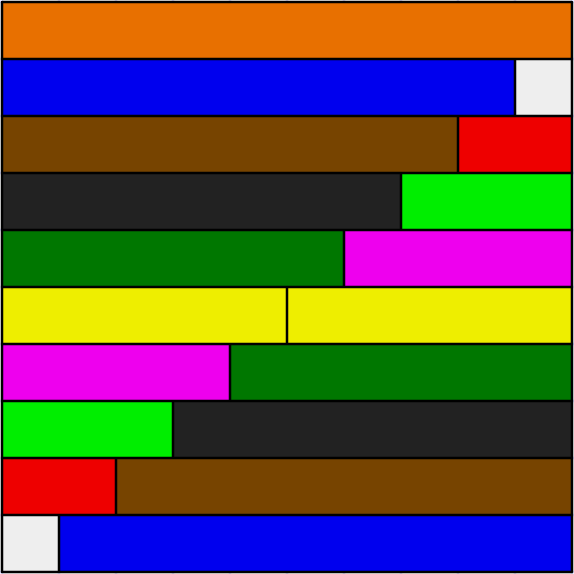
\includegraphics[width=0.3\textwidth]{cuisenaire_combos.png}\\ 
  	\caption{Every number bond to ten using rods}
    \label{fig:cuisenaire_combos}
    \end{center}
\end{figure}

At first, the design of the grid on the board was not quite a grid at all, just a series of rows of contacts for the rods to be placed upon.
Having studied principles of interaction design, specifically the work of cognitive scientist and usability engineer Donald Norman, it became clear that the design would need to be altered so that it would become more obvious how to use the product. In his book, \emph{The Design of Everyday Things} \cite{donaldnorman2002}, Norman talks about `affordances', which are the action possibilities that are readily perceivable by the actor. In the same way that the handle of a cup \emph{affords} grasping it, the design of our board must \emph{afford} the placement of rods in line with the grid squares, in the correct orientation.

In order to achieve this, extra markings were added to the design to demarcate the grid squares. Recessed lines run between columns of squares, to make clear where each column exists, and protruding lines run between the rows of squares, not only as markings, but also serving the purpose of preventing rods being placed in the incorrect orientation to connect different rows, as this may produce incorrect data. 

The comparison of the board before and after these affordances were added in Figures \ref{fig:boardlid_nolines} and \ref{fig:boardlid}  show how effective the markings are in improving the design.

\begin{figure}[H]
	\begin{center}
	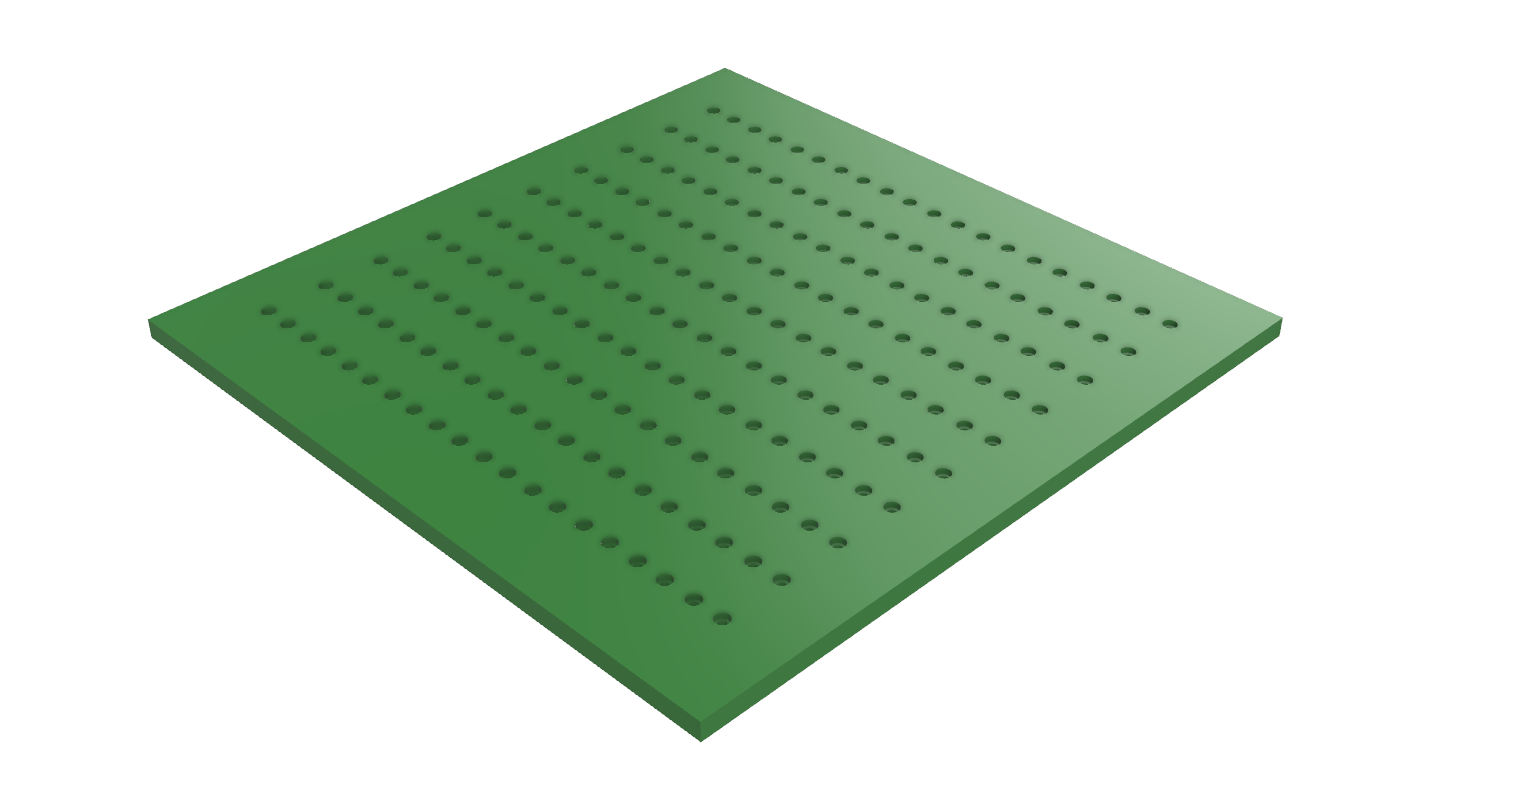
\includegraphics[width=0.75\textwidth]{boardlid_nolines.png}\\ 
  	\caption{Grid squares before markings}
    \label{fig:boardlid_nolines}
    \end{center}
\end{figure}

\begin{figure}[H]
	\begin{center}
	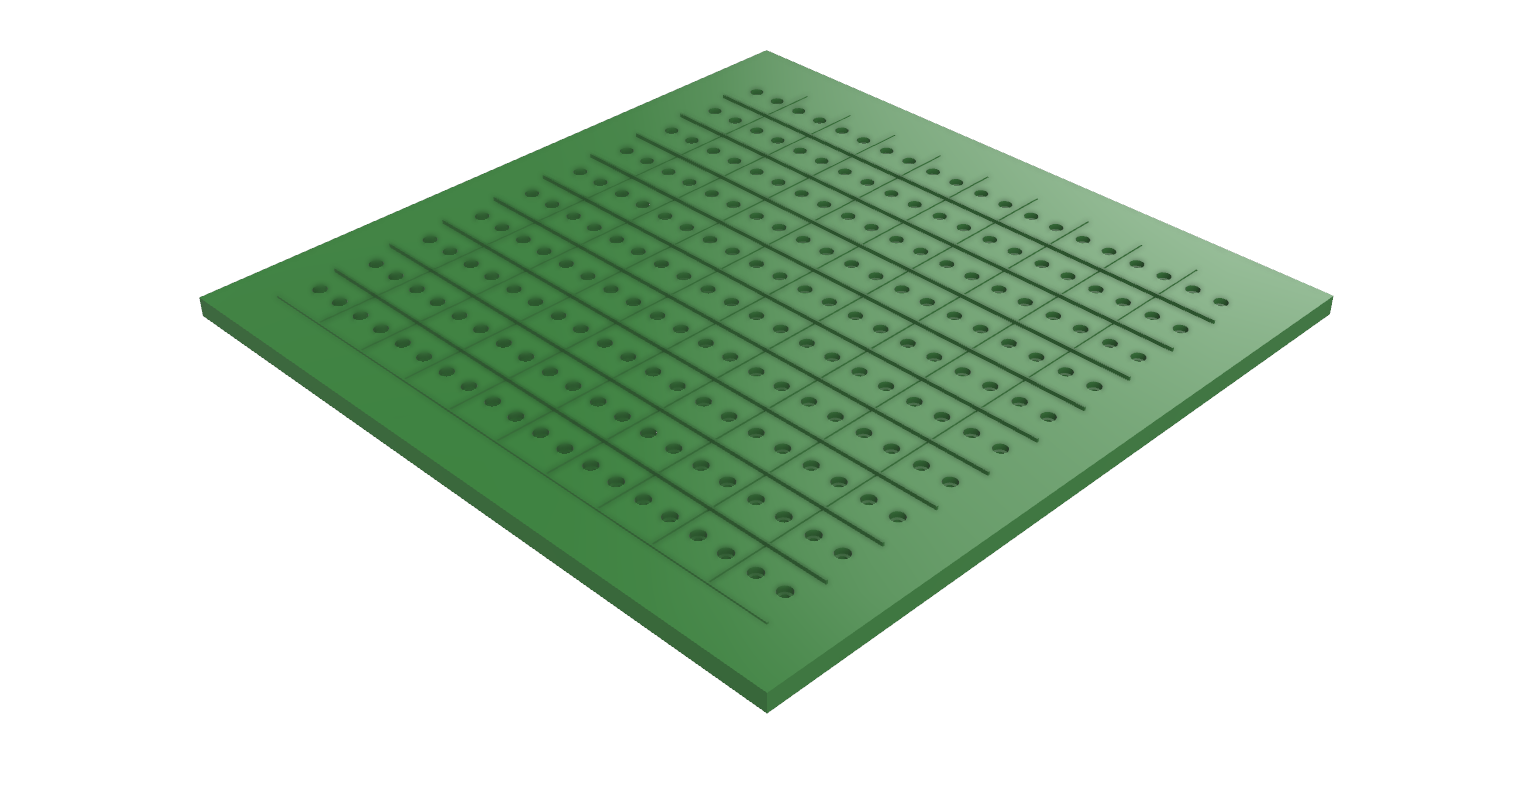
\includegraphics[width=0.75\textwidth]{boardlid.png}\\ 
  	\caption{Grid squares after markings}
    \label{fig:boardlid}
    \end{center}
\end{figure}




\subsection{Circuitry Containment and Interfaces}
\todo[inline]{To Do: Explanation of design of charging port and how circuitry is kept in place}

\section{Software}
\todo[inline]{To Do: Explanation of rod-detecting code}

This section will explain the code that the Arduino uses to interpret voltages read from the multiplexers and determine in what positions rods have been placed. In general terms, the code takes advantage of the fact that connected nodes will be at the same voltage level, so it sweeps along each row, checking to see where adjacent nodes are at equal voltage. The length of consecutive equal nodes corresponds to the length of the rod that has been placed. Note that the following explanations pertain to the code used to control the reduced proof-of-concept circuit, but the the code for the full circuit is very similar, with the exception of extra iterations added to account for the increased number of multiplexers. A listing intended for the full circuit can be found at ------------ but since it was not possible to properly test that code, it cannot definitively be said that it is functional, so the reduced version is explained instead.


\todo[inline]{Mention this is the code for one line and the other code is equivalent ant can be found at ...}

The code begins with global definitions, including the definition of the Arduino GPIO output pins used to  control the select lines of the multiplexers (Figure \ref{lst:mux_sel}). The multiplexers that are directly connected to the resistor chain are referred to as the level 2 multiplexers, and the multiplexer that funnels the level 2 outputs to the Arduino input is the level 1 multiplexer. This resembles their relative positions in the circuit diagram. All the level 2 units are fed the same select input, and the level 1 selects which of those to output to the Arduino, which is why all the multiplexers on the same level have the same select inputs.

\begin{figure}[H]
\centering
\begin{minted}{c++}
// Higher level = closer to resistors
// Lower level = closer to Arduino
unsigned level2_sel[] = { /*lsb*/ 25, 26, 27 /*msb*/ }; 
unsigned level1_sel[] = { /*lsb*/ 22, 23, 24 /*msb*/ };
\end{minted}
\caption{Definition of pins used to control multiplexer select lines }
\label{lst:mux_sel}
\end{figure}

The main body of the code (Figure \ref{lst:read_voltages}) begins by iterating over every node in the chain of resistors, reading the voltage at that node, and storing those values in a two-dimensional array, \texttt{voltages}, where each row of the array corresponds to a row of the board. Note that the iteration is performed in terms of \texttt{NO\_OF\_LINES} and \texttt{NODES\_PER\_LINE}, which are preprocessor variables that can be edited pre-compilaton. This allows the code to extend to boards of any size, should the need arise in the future. \\

The expression in the condition of the innermost for loop, \texttt{j < 8 \&\& (i*8 + j) < NODES\_PER\_LINE} is necessary because there are three level 2 multiplexers per row of resistors, which means a maximum of 24 readings can be made (8 per multiplexer). However, since our circuit only requires readings of 20 nodes, this expression makes sure that the iteration ends after 20, or whatever value \texttt{NODES\_PER\_LINE} may have. In addition, the reason the reading is multiplied by \texttt{(INPUT\_VOLTAGE / 1023.0)} is that \texttt{analogRead()} returns a value that has been processed by a 10-bit analogue-digital converter (ADC), so returns a value between 0 and $2^{10}-1$ (1023), representing multiples of 4.9mV increments from 0V to 5V, and multiplying by this factor converts the value back to a voltage.

\begin{figure}[H]
\centering
\begin{minted}{c++}
// For each line
  for (unsigned line = 0; line < NO_OF_LINES; line++)
  {
      // For each muliplexer
     for (unsigned i = 0; i < 3; i++)
     {
        // Set the select of the level1 mux to the desired level2 output
        digitalWrite(level1_sel[0], (line*3 + i) & 0x1); // Bitmask bit 1
        digitalWrite(level1_sel[1], (line*3 + i) & 0x2); // Bitmask bit 2
        digitalWrite(level1_sel[2], (line*3 + i) & 0x4); // Bitmask bit 3

        // For each input to the level2 multiplexer
        // (Can make 24 reads on level 2 with 3 muxes, but we are only using NODES_PER_LINE of them)
        for (unsigned  j = 0; j < 8 && (i*8 + j) < NODES_PER_LINE; j++) 
        {
          // Set select to that input
          digitalWrite(level2_sel[0], j & 0x1); // Bitmask bit 1
          digitalWrite(level2_sel[1], j & 0x2); // Bitmask bit 2
          digitalWrite(level2_sel[2], j & 0x4); // Bitmask bit 3

          // Take reading, store in respective array element
          voltages[line][(i*8 + j)] = analogRead(output) * (INPUT_VOLTAGE / 1023.0);
        }
      }
    }
\end{minted}
\caption{Reading voltages from resistor chains}
\label{lst:read_voltages}
\end{figure}

Once the \texttt{voltages} structure has been populated, it is converted to a format that shows the state of the board in terms of rod placement, rather than voltage values. This new data structure, \texttt{rods}, has the same dimensions as \texttt{voltages}, but each element is an integer, corresponding to the length of rod currently at that position. For example, a row with a 2-rod, an empty unit space, two consecutive 3-rods, and a unit rod, as in Figure \ref{fig:example_row}, would be denoted as 


$$\texttt{[2, 2, 0, 3, 3, 3, 3, 3, 3, 1].}$$


The value at that element of the array denotes the length of rod occupying that position, and since the value is repeated according to the number of positions the rod occupies, it is possible to discern the rod's length. Even though it may seem difficult to calculate where the two 3-rods are since they are adjacent, using this knowledge and reading the array left-to-right allows to identify where they both begin and end. The 0 value indicates an empty position. \\

\begin{figure}[H]
	\begin{center}
	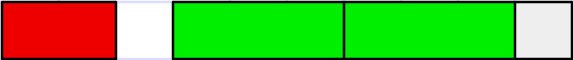
\includegraphics[width=0.3\textwidth]{example_row.png}\\ 
  	\caption{An example row of rods}
    \label{fig:example_row}
    \end{center}
\end{figure}

The program detects whether nodes are connected by a rod by reading the \texttt{voltages} structure, checking to see if their voltages are the same (within a small margin, to account for slight differences due to the impedances of the multiplexers and the tolerance of the resistors). The number of consecutive nodes at the same voltage is indicative of the size of the rod which has been placed. For example, a unit rod would short two nodes, whereas a 6-rod would short twelve adjacent nodes. 

Once the positions of rods has been determined, the newly-calculated state is compared to the previous state to identify changes. If there has been a change of state (in other words, if a rod has been placed or removed), then the new state is saved for future comparisons, and is communicated to the web app. This functionality is detailed further in Section \ref{sec:hub_comms}.

\section{Circuit}

\subsection{Choosing a resistor value}
% Requirements + model + simulation
The circuit can be described as 10 parallel chains of identical resistors, with a series of multiplexers reading the voltage at every node, funnelling those values to an analogue input on the Arduino. \\

As mentioned in Section \ref{sec:conductivematerial}, the value of the resistors is important, as picking a value too high will cause the current to drop to unmeasurable levels. However, a resistance too low will draw unnecessary power, which should be avoided, since this is a portable product, and is powered by a limited battery. \\

The datasheet \cite{CD405xBC19:online} of the multiplexer the circuit uses states that, typically, $0.04\mu{}A$ is needed for a reading. Therefore, the circuit needs to use a resistor such that each node being read by a multiplexer has at least that much current flowing through it, while still trying to maximise the resistance to minimise power drawn.\\

To find the value of this resistor, a model of the circuit was created, and a simulation run, which calculates the resistance at which these conditions are satisfied. \\

\todo[inline]{To Do: Explanation of and results of simulation, including circuit diagram}

The choice was made to produce the final circuit by soldering through-hole components to a stripboard, rather than using printed circuit boards (PCBs). This was a precautionary measure, in anticipation of changes that would need to be made as problems arose. Advice from V. Boddy, the Project Lab Manager, revealed that PCBs could take from 5-15 days to be produced and delivered, and could cost upwards of hundreds of pounds, depending on speed of delivery. Speaking with Prof. Constantinides also led to the same conclusion that stripboard would be a happy compromise of permanence and reconfigurability, reducing reliance on third parties and keeping costs low.\\

However, in hindsight, this may have not been the correct decision. It seems that in these discussions the full extent of the complexity of the circuit was not foreseen. The full circuit requires 10 chains of 21 resistors, with each node connected to a multiplexer. This requires 36 multiplexers, each of which require connections to power rails as well as select inputs. This alone accounts for almost 300 flying leads and over 1000 solder joints. This does not include the soldering that would need to be done to connect the resistors to the contacts on the board, which would add several hundred more solder joints. \\

Work on the circuit reached about halfway when it was realised that it would not be wise to carry on. Firstly, with the amount of manual soldering required, it became increasingly likely that an error would occur, even with regular continuity tests, which may render the circuit unusable. This was unacceptable due to the amount of time it took to build the circuit. Around two weeks were spent bringing the circuit to that halfway point, much of which was spent manually cutting and stripping wires. Additionally, although care was taken to organise cables neatly, the amount of cabling required made for a confusing and tangled circuit, to which it became increasingly difficult to add more cables. Figure \ref{fig:wiring} shows the circuit in its current state, and should make it clear why work was discontinued. Using a PCB would have removed the need for the flying leads, and even if it took several days for a new print to arrive, those days could be used doing other work, so would not be wasted.\\

In lieu of the full circuit, a reduced version was produced to be used as a proof-of-concept for demonstration purposes. This reduced circuit carries the same functionality as the full circuit but only for one chain of resistors -- in other words, one row of the board. The design is very scalable, and demonstration that one row functions properly is enough to showcase the abilities of the full circuit. The only difference is that with more rows added, the current drawn is increased, so after a certain number of rows are added, the Arduino will no longer be able to supply enough current to power the device.


\begin{figure}[H]
	\begin{center}
	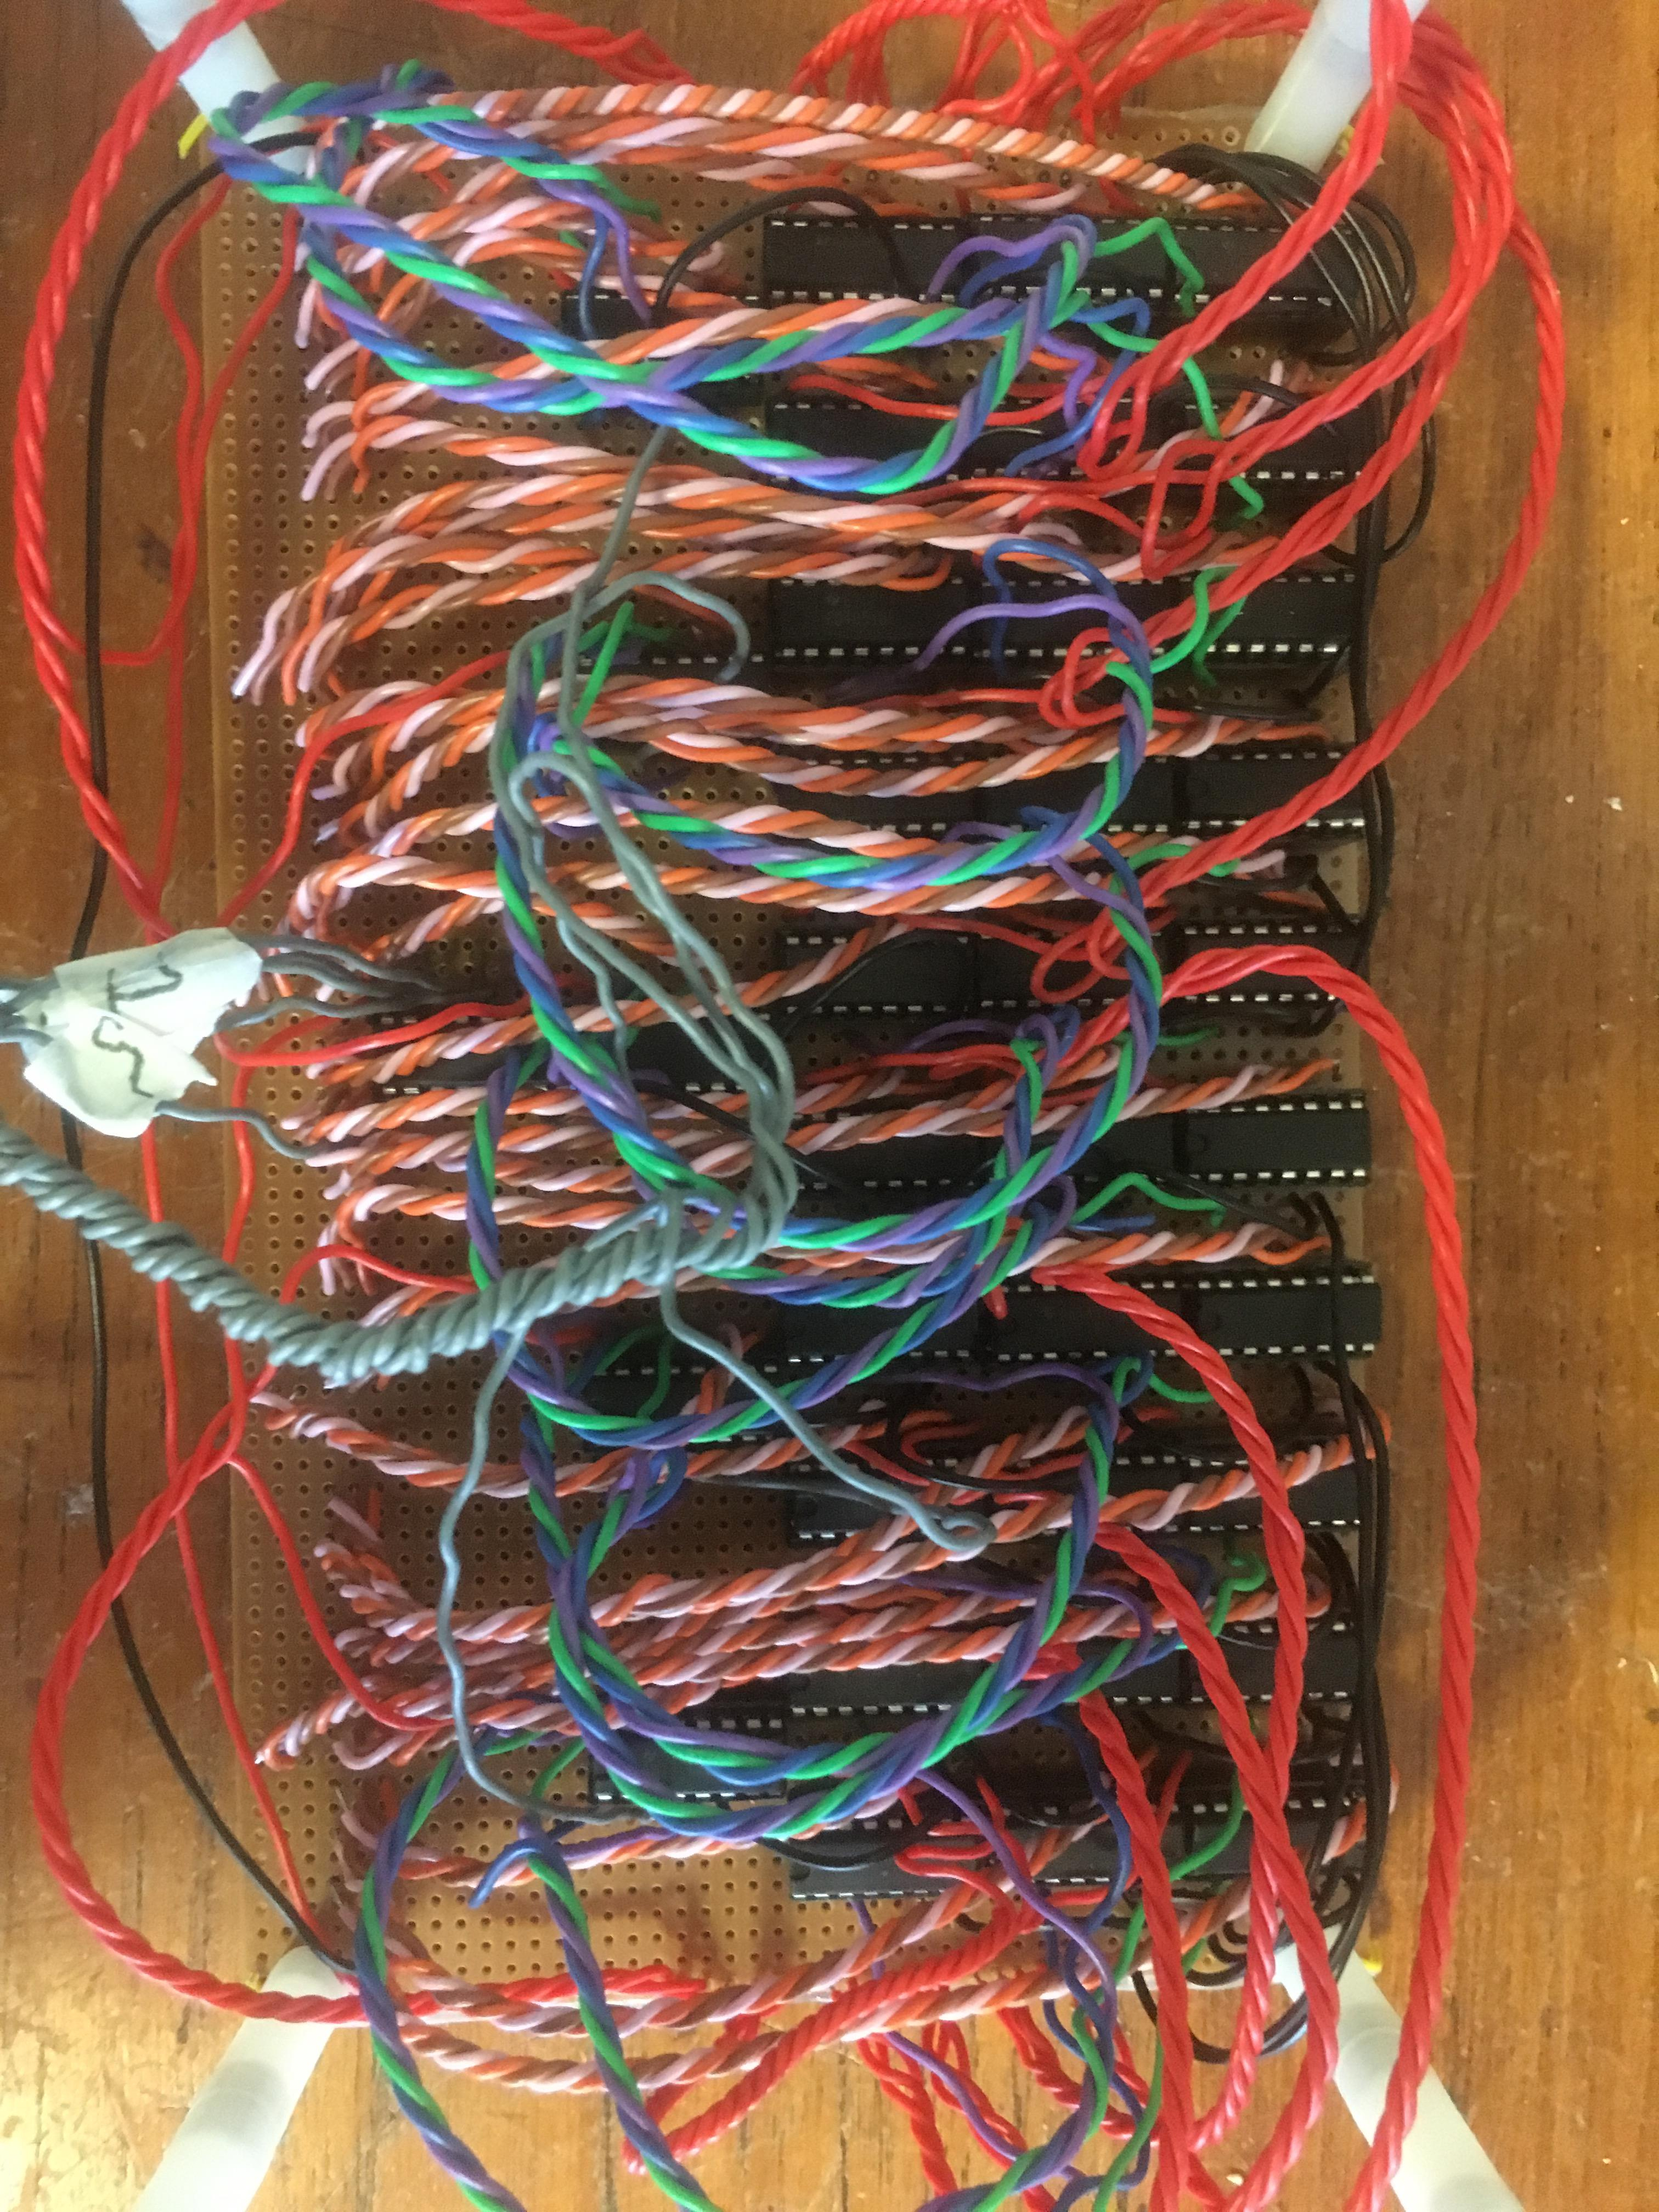
\includegraphics[width=0.5\textwidth, angle=270]{wiring.JPG}\\ 
  	\caption{Circuit partially made using stripboard}
    \label{fig:wiring}
    \end{center}
\end{figure}

\todo[inline]{To Do: Discuss creation of circuit on stripboard and connection of resistors to multiplexers}

	% Choice to use multiplexers + why that multiplexer
    % Finding input impedance of mux and how to choose resistor size
   	% Positioning of component to slot into lid
    % layers of stripboard
    % Choice to use stripboard and not PCB (flexibility in changes)

\subsection {Resistor Layout}

The orientation and layout of the resistors went through several design iterations. 

\section{Power}

The choice was made to make the product battery-powered, to improve accessibility for users. If mains powered, a class would need dozens of power cables and likely also extension cords. These are an inconvenience for the class and also pose a tripping hazard, with so many wires being used.\\

To make charging the device easy, a rechargeable lithium-ion battery in conjunction with an Adafruit Powerboost 500c \cite{PowerBoo78:online} are used. The Powerboost connects to the battery and also provides a USB port with a 5.2V output to power the Arduino, as well as a microUSB port that can be used to charge the battery or power the device directly. MicroUSB  is a very commonly used interface, meaning that it will not be difficult for users to replace charging cables. 


	% Why portable/battery powered
    

\section{Board to Hub Communication}
\label{sec:hub_comms}
\todo[inline]{To Do: Explain usage of radio transceiver that failed and new bluetooth module, including communication protocol used}
	% nRF24L01 failure
    % HC05 success
    	% Talk about recommendations from internet forums as source
    % What data is sent and in what format and why

	% What data is sent from rpi to server and in what format and why
    
    
    
    
    
\chapter{Testing}
\chapter{Results Analysis}
\chapter{User Guide}

\bibliography{references.bib}
\bibliographystyle{ieeetr}

\begin{appendix}
\chapter{1}



\end{appendix}

\end{document}